\chapter{Implementacja}
%W tej części pracy zostanie omówiona implementacja systemu eBOKa „Harmony Home Net”. 
Proces implementacji polega na przełożeniu założeń architektonicznych, wymagań funkcjonalnych oraz niefunkcjonalnych na działający kod, a także integracji poszczególnych komponentów systemu w spójną całość. W przypadku systemu eBOKa „Harmony Home Net” proces ten obejmuje zarówno warstwę frontendową, odpowiadającą za interakcje użytkowników, jak i backend, zajmujący się logiką biznesową i zarządzaniem danymi. Kluczowym elementem implementacji jest integracja z bazą danych PostgreSQL uruchomioną w środowisku Docker.

% TO DO: praca wymaga poprawek stylistycznych. Niektóre zdania są "zbyt pompatyczne", czasem też niegramatyczne.
Warto podkreślić, że obecnie system „Harmony Home Net” ma charakter prototypu. Pozwala on na walidację podstawowych założeń oraz funkcji aplikacji eBOK, jednocześnie stanowiąc fundament dla przyszłego rozwoju pełnoprawnej aplikacji produkcyjnej. Zastosowane technologie, takie jak Next.js dla frontendu, Spring Boot dla backendu oraz Docker dla konteneryzacji, zapewniają skalowalność oraz łatwość rozbudowy systemu w kolejnych etapach.

Rozdział rozpocznie omówienie zastosowanej \textbf{architektury warstwowej}~\cite{n_tier_wiki}, która jest podstawą projektowanego systemu. Szczegółowo opisane zostaną wszystkie warstwy – prezentacji, logiki biznesowej oraz dostępu do danych – z uwzględnieniem ich ról oraz sposobu implementacji. Następnie uwaga zostanie zwrócona na \textbf{bazę danych}. Omówione zostaną podejścia \emph{Database First} i \emph{Code First}, wraz z uzasadnieniem wyboru pierwszego z nich. Podane zostaną szczegóły zaprojektowanej struktury bazy danych oraz sposób jej integracji z aplikacją.

Przegląd kluczowych elementów systemu związanych z \textbf{bezpieczeństwem} obejmie mechanizmy autoryzacji i uwierzytelniania, zrealizowane za pomocą Spring Security. Następnie zostanie opisane \textbf{zarządzanie użytkownikami systemu}, a także inne istotne funkcje, jak zarządzanie mieszkaniami, zgłoszeniami technicznymi, płatnościami i powiadomieniami.


% TO DO: czy rzeczywiście wdrożenia? Wdrożenie to proces instalacji i uruchomienia aplikacji w środowisku produkcyjnym.
%        lekko przeredagowując można poniższe zdania przenieść do Układu pracy
%Celem tej części pracy jest nie tylko opisanie kroków wdrożenia, ale również ukazanie, w jaki sposób zaimplementowane rozwiązania odpowiadają na postawione wymagania funkcjonalne i niefunkcjonalne. Rozdział kończy się krótkim podsumowaniem, które ocenia, jak wdrożone funkcjonalności wpisują się w założenia projektu oraz wskazuje potencjalne kierunki dalszego rozwoju aplikacji.


\section{Architektura warstwowa}

Architektura warstwowa jest jednym z najbardziej rozpowszechnionych wzorców projektowych w inżynierii oprogramowania. Polega na podziale aplikacji na logiczne warstwy, z których każda pełni określoną funkcję. W typowej architekturze warstwowej wyróżnia się cztery kluczowe warstwy: warstwę prezentacji, logiki biznesowej, dostępu do danych oraz warstwę danych~\cite{n_tier_baeldung, n_tier_medium}. Ich ogólny schemat przedstawiono na rysunku \ref{fig:n_tier_arch}. Poszczególne elementy schematu oznaczono literami (a, b, c, d), co pozwala na ich jednoznaczną identyfikację w dalszym opisie.

\noindent Podział na warstwy przynosi wiele korzyści:
\begin{itemize}
    \item \textbf{Modularność} -- niezależność warstw ułatwia rozwój i utrzymanie systemu.
    \item \textbf{Reużywalność} -- komponenty warstw mogą być łatwo wykorzystane w innych projektach.
    \item \textbf{Skalowalność} -- warstwy można skalować oddzielnie, co zwiększa elastyczność aplikacji.
    \item \textbf{Czytelność kodu} -- podział odpowiedzialności sprawia, że kod jest bardziej przejrzysty.
    \item \textbf{Testowalność} -- warstwy mogą być testowane oddzielnie, co ułatwia identyfikację błędów.
\end{itemize}
Do wad architektury warstwowej należą:
\begin{itemize}
    \item \textbf{Potencjalny narzut} -- dodatkowe poziomy abstrakcji mogą obniżyć wydajność systemu.
    \item \textbf{Złożoność implementacji} -- koncepcja ma być bez nadmiernego zagnieżdżania warstw.
    \item \textbf{Brak elastyczności} -- w pewnych scenariuszach może być trudno dostosować architekturę do nietypowych wymagań.
\end{itemize}

Zastosowanie architektury warstwowej w systemie „Harmony Home Net” zapewnić ma jego modularność, skalowalność oraz łatwość utrzymania, spełniając wymagania zarówno użytkowników końcowych, jak i administratorów.
\begin{figure}[htb]
    \centering
    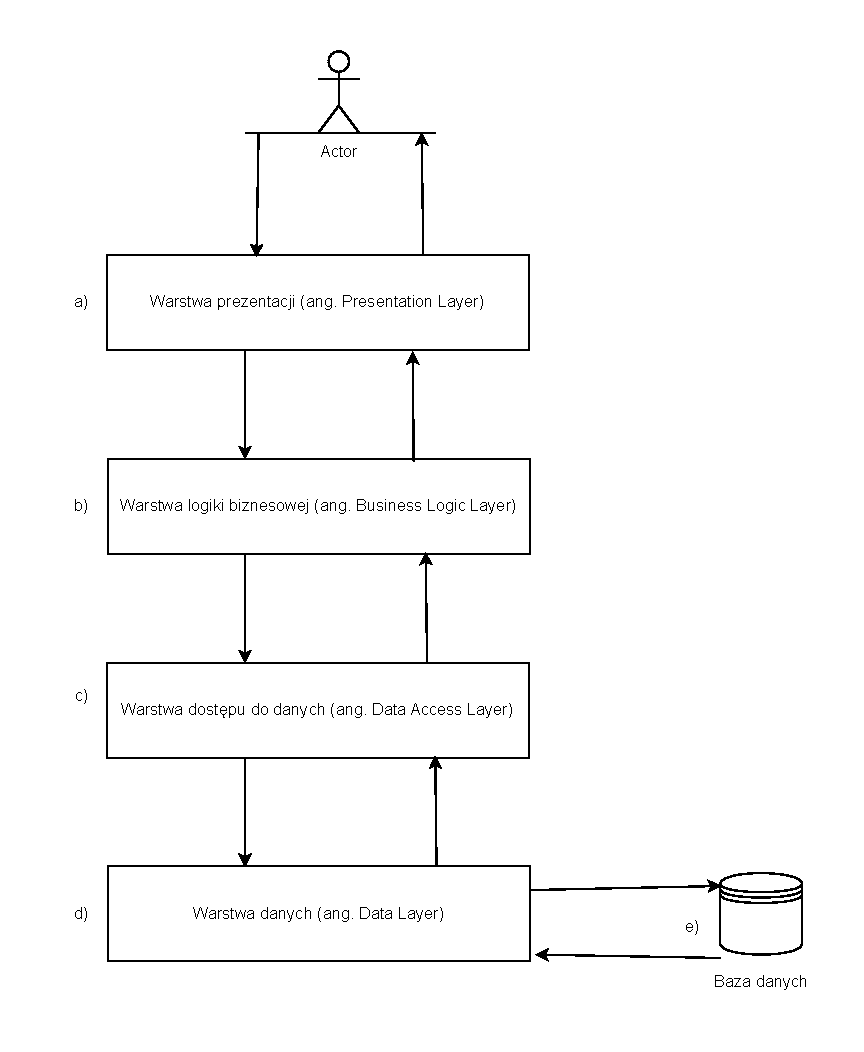
\includegraphics[scale=1.2]{rys03/diagram_architektury_warstwowej}
    \caption{Ogólny schemat architektury warstwowej}
    \label{fig:n_tier_arch}
\end{figure}

\subsection{Warstwa prezentacji (ang.\ \emph{Presentation Layer})}
Warstwa prezentacji, oznaczona literą \texttt{a)} na rysunku \ref{fig:n_tier_arch}), odpowiada za interakcję użytkownika z systemem. Na tym poziomie użytkownik wprowadza dane wejściowe, a system zwraca wyniki w formie czytelnej i zrozumiałej. Głównym zadaniem warstwy prezentacji jest renderowanie interfejsu użytkownika oraz obsługa zdarzeń takich jak kliknięcia czy przesunięcia. Odpowiada również za wstępną walidację danych wejściowych, na przykład sprawdzanie, czy wprowadzony adres e-mail ma poprawny format. Przetworzone dane są następnie przekazywane do warstwy logiki biznesowej, gdzie są dalej analizowane i przetwarzane.

W warstwie prezentacji zastosowano również architekturę typu AJAX. Jest to technologia umożliwiająca komunikację między przeglądarką użytkownika a serwerem w sposób asynchroniczny, co oznacza, że wymiana danych może zachodzić bez konieczności przeładowania całej strony. Dzięki temu interfejs użytkownika pozostaje dynamiczny i responsywny~\cite{ajax}.

Mechanizm działania AJAX jest następujący:
\begin{itemize}
    \item Gdy użytkownik wykonuje określoną akcję (np. klika przycisk), przeglądarka wysyła żądanie HTTP do serwera za pomocą obiektu \texttt{XMLHttpRequest} lub współczesnych API takich jak \texttt{fetch}.
    \item Serwer przetwarza żądanie i zwraca odpowiedź, najczęściej w formacie JSON, który jest łatwy do przetwarzania po stronie klienta.
    \item Warstwa prezentacji przetwarza otrzymane dane i aktualizuje odpowiednie elementy strony bez konieczności jej ponownego ładowania.
\end{itemize}

Przykładowym zastosowaniem AJAX w systemie „Harmony Home Net” jest dynamiczne odświeżanie listy ogłoszeń, płatności czy zgłoszeń technicznych w zależności od akcji użytkownika. Dzięki temu użytkownik otrzymuje aktualne dane w czasie rzeczywistym, co znacząco poprawia komfort pracy z systemem.


W systemie ,,Harmony Home Net,, warstwę tę zrealizowano za pomocą frameworka Next.js, w~języku TypeScript. Odpowiada ona za wyświetlanie interfejsu użytkownika, w tym panelu właściela, gdzie użytkownicy mogą przeglądać zgłoszenia techniczne, dokonywać płatności oraz uczestniczyć w głosowaniach. Użycie Next.js umożliwia renderowanie po stronie serwera, co poprawia wydajność aplikacji oraz jej pozycjonowanie w wyszukiwarkach (SEO). Dzięki komponentom wielokrotnego użytku interfejs użytkownika jest spójny wizualnie i funkcjonalnie. 

\subsection{Warstwa logiki biznesowej (ang.\ \emph{Business Logic Layer})}

Warstwa logiki biznesowej, oznaczona  literą \texttt{b)} na rysunku \ref{fig:n_tier_arch}, pełni kluczową rolę w przetwarzaniu danych wejściowych i realizacji reguł biznesowych. Na tym poziomie dane są analizowane i przetwarzane zgodnie z zasadami określonymi przez specyfikę aplikacji. Główne zadania tej warstwy obejmują koordynację przepływu danych między innymi warstwami oraz obsługę wyjątków, które mogą wystąpić w wyniku błędów na wcześniejszych etapach przetwarzania.

W~systemie ,,Harmony Home Net'' warstwa ta, oparta na Spring Boot, realizuje procesy biznesowe takie jak autoryzacja użytkowników przy użyciu OAuth 2.0, zarządzanie zgłoszeniami technicznymi oraz integracja z systemami płatności. Warstwa ta komunikuje się z frontendem poprzez REST API, co zapewnia efektywne przetwarzanie żądań i odpowiedzi. Dodatkowo technologia Spring Boot umożliwia implementację skalowalnych i bezpiecznych rozwiązań, co jest kluczowe w przypadku obsługi dużej liczby użytkowników.

\subsection{Warstwa dostępu do danych (ang.\ \emph{Data Access Layer})}

Warstwa dostępu do danych, oznaczona literą \texttt{c)} na rysunku \ref{fig:n_tier_arch}, odpowiada za komunikację między logiką biznesową a fizycznym przechowywaniem danych. Jej główną funkcją jest wykonywanie operacji takich jak zapisywanie, odczytywanie, aktualizowanie i usuwanie danych w sposób zoptymalizowany i bezpieczny. Często korzysta się z bibliotek ORM, takich jak Hibernate lub JPA w Javie, które ułatwiają mapowanie danych między bazą a obiektami aplikacji.

W systemie ,,Harmony Home Net,, baza danych PostgreSQL została uruchomiona w środowisku Docker. Dzięki zastosowaniu JPA możliwe jest łatwe mapowanie danych między tabelami bazodanowymi a obiektami aplikacji w Javie. Taka implementacja umożliwia optymalizację zapytań i zapewnia wydajność operacji, co jest istotne w przypadku dużej ilości danych przechowywanych w systemie, takich jak zgłoszenia techniczne czy płatności właścieli.

\subsection{Warstwa danych (ang.\ \emph{Data Layer})}
Warstwa danych, oznaczona literą \texttt{d)} na rysunku \ref{fig:n_tier_arch}, odpowiada za trwałe przechowywanie danych aplikacji w bazach danych. Obejmuje zarządzanie strukturą danych, ich bezpieczeństwem oraz udostępnianie ich innym warstwom w sposób wydajny i zorganizowany. W systemie ,,Harmony Home Net'' wykorzystano bazę danych PostgreSQL wdrożoną w kontenerze Docker. 

Projektowanie bazy danych to jeden z kluczowych etapów tworzenia systemów informatycznych. Może odbywać się w podejściach \emph{Database First} i \emph{Code First}~\cite{DB_FIRST_VS_CODE_FIRST_1,DB_FIRST_VS_CODE_FIRST_2}. 

Podejście \emph{Code First} zakłada, że na początku w kodzie aplikacji powstanie model danych. Następnie na podstawie tego kodu zostanie wygenerowany schemat bazy danych~\cite{CODE_FIRST}. Dzięki temu podejściu możliwe są dynamiczne zmiany w~strukturze danych podczas rozwoju aplikacji. Przydaje się to w projektach, gdzie schemat bazy danych ewoluuje w odpowiedzi na zmieniające się wymagania biznesowe. Jednak w dużych projektach, w których schemat danych jest złożony i~wymaga precyzyjnej kontroli, podejście to może nie zadziałać.

Podejście \emph{Database First} polega na zaprojektowaniu schematu bazy danych, a następnie wygenerowaniu modelu aplikacji na jego podstawie. Jest to podejście bardziej tradycyjne, dające większą przewidywalność i precyzję, co jest istotne w systemach o wysokim stopniu zależności od integralności danych. Dodatkowo pozwala na pełne wykorzystanie możliwości narzędzi ORM, takich jak JPA, ponieważ bazuje na uprzednio zaprojektowanym schemacie. 

Dzięki zastosowaniu mapowania ORM dane w bazie są bezpośrednio odwzorowywane na obiekty w aplikacji, co pozwala na wygodniejsze operacje na danych. Mechanizm ORM umożliwia wykonywanie zapytań SQL w sposób abstrakcyjny i bardziej czytelny, co upraszcza implementację i zmniejsza ryzyko błędów.

\section{Struktura bazy danych}
W kontekście systemu ,,Harmony Home Net'' zdecydowano się na podejście \emph{Database First}. Zdecydowano się na to z kilku ważnych powodów.
\begin{itemize}
    \item \textbf{Centralna rola bazy danych} -- baza danych pełni kluczową funkcję w systemie, przechowując informacje o użytkownikach, lokalach, zgłoszeniach technicznych oraz płatnościach. Precyzyjne zaprojektowanie jej struktury na etapie początkowym pozwoliło na lepsze zrozumienie relacji między danymi i~ich hierarchii.
    \item \textbf{Integracja z narzędziami ORM} -- dzięki wykorzystaniu podejścia \emph{Database First}, istniejące narzędzia ORM, takie jak JPA (Java Persistence API), mogły zostać bezproblemowo dostosowane do uprzednio przygotowanego schematu bazy danych, co uprościło implementację i~zmniejszyło ryzyko błędów.
    \item \textbf{Zgodność z wymaganiami aplikacji} -- rozpoczęcie od projektowania bazy danych zapewniło uzyskanie zgodności struktury danych z wymaganiami funkcjonalnymi i niefunkcjonalnymi. Umożliwiło również identyfikację potencjalnych problemów na wczesnym etapie prac.
    \item \textbf{Bezpieczeństwo i integralność danych} -- projektując bazę danych jako pierwszą można było od razu uwzględnić mechanizmy zabezpieczeń, takie jak klucze główne, obce oraz indeksy. Zminimalizowało to ryzyko wystąpienia niespójności danych w trakcie działania systemu.
\end{itemize}

\subsection{Opis struktury}

Strukturę bazy danych w systemie „Harmony Home Net” zaprojektowano z uwzględnieniem wymagań funkcjonalnych i niefunkcjonalnych aplikacji. Schemat bazy danych podzielono na warstwę konceptualną (rysunek \ref{fig:ebok_db_concept}) oraz fizyczną (rysunek \ref{fig:ebok_db_physical}), co umożliwiło dokładne odwzorowanie relacji pomiędzy danymi oraz optymalizację ich przechowywania.
\begin{figure}[ht]
    \centering
    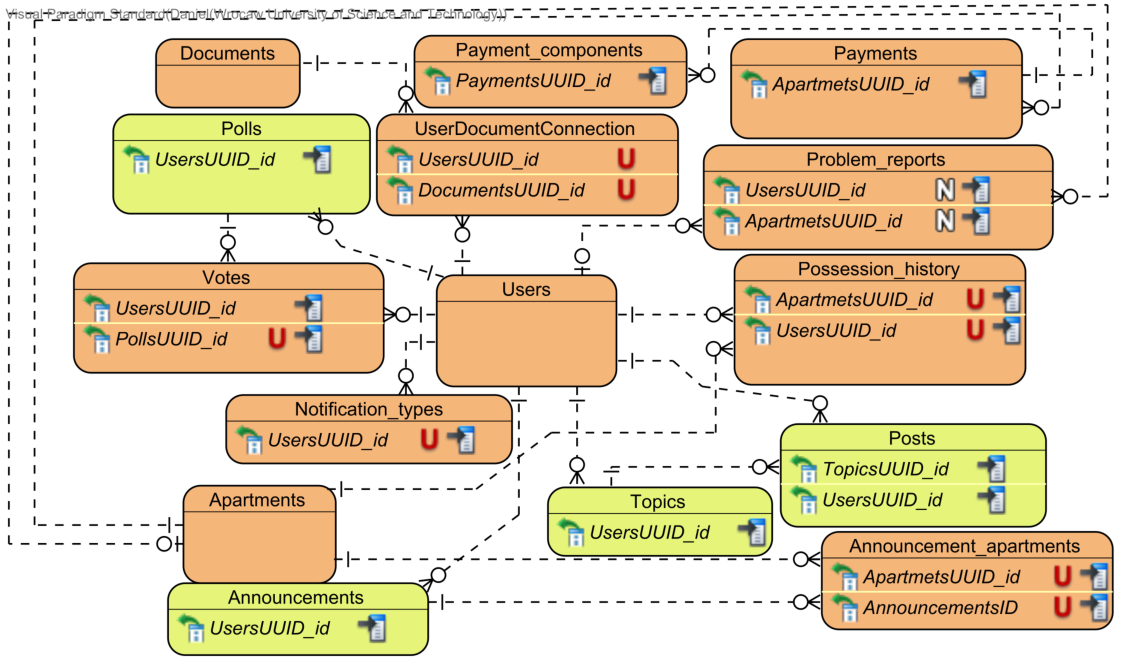
\includegraphics[width=.9\linewidth]{rys03/ebok_db_concept}
    \caption{Schemat konceptualny bazy danych systemu}
    \label{fig:ebok_db_concept}
\end{figure}
\begin{figure}[ht]
    \centering
    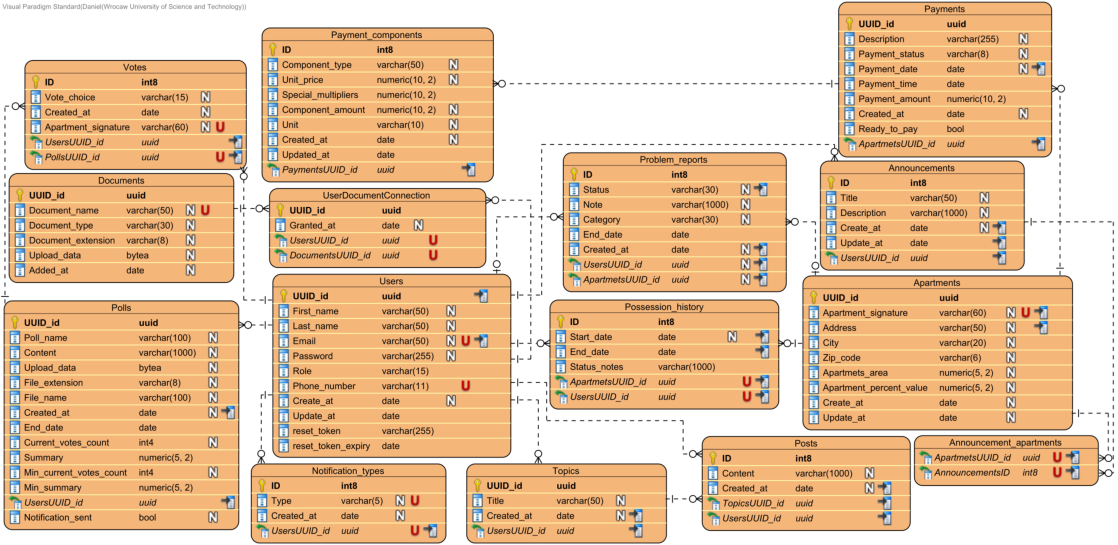
\includegraphics[width=1\linewidth]{rys03/ebok_db_physical}
		\caption{Schemat fizyczny bazy danych systemu}
    \label{fig:ebok_db_physical}
\end{figure}

\subsubsection{Opis tabel}
Poniżej szczegółowo opisano wszystkie tabele w bazie danych:

\begin{itemize}
    \item \textbf{Tabela \texttt{Users}:}
    Przechowuje dane o użytkownikach, takie jak:
    \begin{itemize}
        \item \texttt{FirstName} i \texttt{LastName} -- imię i nazwisko użytkownika,
        \item \texttt{Email} -- unikalny adres e-mail,
        \item \texttt{Password} -- zaszyfrowane hasło,
        \item \texttt{Role} -- rola w systemie (np. właściciel, pracownik, administrator),
        \item \texttt{CreateAt} i \texttt{UpdateAt} -- daty utworzenia i ostatniej modyfikacji rekordu.
    \end{itemize}
    Klucz główny \texttt{UUID} jest wykorzystywany jako klucz obcy w wielu innych tabelach, zapewniając spójność relacji.

    \item \textbf{Tabela \texttt{Apartments}:}
    Zawiera szczegółowe dane o lokalach:
    \begin{itemize}
        \item \texttt{ApartmentSignature} -- unikalny identyfikator lokalu,
        \item \texttt{Address}, \texttt{City} i \texttt{ZipCode} -- adres lokalu,
        \item \texttt{ApartmentArea} -- powierzchnia,
        \item \texttt{ApartmentPercentValue} -- udział procentowy w nieruchomości wspólnej.
    \end{itemize}
    Powiązana z użytkownikami poprzez klucz obcy \texttt{UsersUUID}.
    
    \item \textbf{Tabela \texttt{Payments}:}
    Rejestruje dane o płatnościach:
    \begin{itemize}
        \item \texttt{Description}, \texttt{PaymentStatus}, \texttt{PaymentDate}, \texttt{PaymentAmount},
        \item \texttt{ReadyToPay} -- znacznik stanu płatności.
    \end{itemize}

    \item \textbf{Tabela \texttt{PaymentComponent}:}
    Szczegółowo opisuje składniki płatności, co pozwala na większą elastyczność w obliczaniu należności. Przechowuje informacje takie jak:
    \begin{itemize}
        \item \texttt{ComponentType} -- typ składnika płatności (np. czynsz, media, fundusz remontowy),
        \item \texttt{UnitPrice} i \texttt{ComponentAmount} -- cena jednostkowa i łączna kwota dla składnika,
        \item \texttt{SpecialMultipliers} -- specjalne mnożniki stosowane w obliczeniach (np. liczba osób, powierzchnia lokalu),
        \item \texttt{Unit} -- jednostka składnika (np. m\textsuperscript{2}, sztuki).
    \end{itemize}
    Tabela jest powiązana z tabelą \texttt{Payments} poprzez klucz obcy \texttt{PaymentsUUID}.

    \item \textbf{Tabela \texttt{ProblemReports}:}
    Zawiera zgłoszenia techniczne dotyczące lokali:
    \begin{itemize}
        \item \texttt{Status}, \texttt{Category}, \texttt{Note} -- szczegóły zgłoszenia,
        \item Klucze obce \texttt{UsersUUID} i \texttt{ApartmentsUUID}.
    \end{itemize}

    \item \textbf{Tabele \texttt{Polls} i \texttt{Votes}:} 
		Obsługują głosowania: tabela \texttt{Polls} zawiera dane głosowań, a \texttt{Votes} przechowuje głosy użytkowników. Wprowadzono ograniczenie unikalności głosów w relacji \texttt{pollId} oraz \texttt{apartmentSignature}.

    \item \textbf{Tabela \texttt{Documents} i \texttt{UserDocumentConnection}:}
    \texttt{UserDocumentConnection} pełni rolę łącznika w relacji wiele do wielu między \texttt{Users} a \texttt{Documents}. Tabela \texttt{Documents} przechowuje informacje o plikach, takie jak nazwa, typ, treść (\texttt{UploadData}) oraz data dodania.
    
    \item \textbf{Tabela \texttt{Announcements} i \texttt{AnnouncementApartment}:}
    \texttt{Announcements} przechowuje ogłoszenia, a \texttt{AnnouncementApartment} pełni rolę tabeli łącznikowej w relacji wiele do wielu między \texttt{Announcements} a \texttt{Apartments}.

    \item \textbf{Tabela \texttt{NotificationTypes}:}
    Przechowuje różne typy powiadomień i ich relacje z użytkownikami. Zdefiniowano ograniczenie unikalności, które uniemożliwia przypisanie tego samego typu powiadomienia temu samemu użytkownikowi wielokrotnie.

    \item \textbf{Tabela \texttt{PossessionHistory}:}
    Rejestruje historię przypisania użytkowników do lokali:
    \begin{itemize}
        \item \texttt{StartDate} i \texttt{EndDate} -- okres użytkowania lokalu,
        \item Klucze obce \texttt{ApartmentsUUID} i \texttt{UsersUUID}.
        \item Zastosowano ograniczenie unikalności relacji między \texttt{userId} a \texttt{apartmentId}.
    \end{itemize}
\end{itemize}

\subsubsection{Podział tabel na pakiety}

W implementacji kodu wszystkie tabele zostały podzielone na dwa logiczne pakiety:
\begin{itemize}
    \item \textbf{Pakiet \texttt{sideTables}:} Obejmuje tabele pomocnicze, które pełnią rolę łączników w relacjach wiele do wielu. Należą do niego:
    \begin{itemize}
        \item \texttt{UserDocumentConnection},
        \item \texttt{PossessionHistory},
        \item \texttt{AnnouncementApartment}.
    \end{itemize}

    \item \textbf{Pakiet \texttt{mainTables}:} Obejmuje główne tabele przechowujące kluczowe dane systemu:
		\begin{multicols}{2}\setlength\topskip{0pt}
    \begin{itemize}
        \item \texttt{Users},
        \item \texttt{Apartments},
        \item \texttt{Payments},
        \item \texttt{PaymentComponent},
        \item \texttt{ProblemReports},
        \item \texttt{Polls},
        \item \texttt{Votes},
        \item \texttt{Documents},
        \item \texttt{Announcements},
        \item \texttt{NotificationTypes}.
    \end{itemize}
		\end{multicols}
\end{itemize}

Podział tabel na dwa pakiety zapewnia przejrzystość struktury kodu, łatwość zarządzania relacjami między encjami oraz ułatwia przyszłą rozbudowę systemu.


\subsection{Więzy integralności oraz wydajność}
Związki między tabelami odwzorowano za pomocą kluczy głównych i obcych, co umożliwia utrzymanie integralności danych. Przykładowo tabela \texttt{Problem\_reports} zawiera klucze obce do tabel \texttt{Users} i \texttt{Apartments}, co pozwala na przypisanie zgłoszeń technicznych zarówno do konkretnego użytkownika, jak i lokalu. Analogicznie, tabela \texttt{Payments} jest powiązana z tabelą \texttt{Apartments}, co zapewnia pełną kontrolę nad płatnościami przypisanymi do danych lokali.

W celu poprawy wydajności bazy danych zastosowano następujące mechanizmy:
\begin{itemize}
    \item \textbf{Indeksy} -- kluczowe kolumny, takie jak \texttt{UUID}, zostały zaindeksowane w celu przyspieszenia operacji wyszukiwania i sortowania.
    \item \textbf{Mapowanie ORM} -- baza danych została zintegrowana z aplikacją za pomocą narzędzia JPA (Java Persistence API), co umożliwia bezpośrednie mapowanie tabel na obiekty w kodzie aplikacji. Dzięki temu operacje CRUD (Create, Read, Update, Delete) mogą być realizowane w sposób wygodny i abstrakcyjny, bez konieczności pisania zapytań SQL.
    \item \textbf{Konteneryzacja} -- PostgreSQL działa w środowisku Docker, co zapewnia łatwość zarządzania i możliwość skalowania systemu w zależności od obciążenia.
		\item \textbf{Ograniczenia unikalności (ang. Unique Constraint)} -- w tabelach takich jak \texttt{Votes}, \texttt{PossessionHistory}, \texttt{NotificationTypes}, oraz \texttt{AnnouncementApartment} zastosowano ograniczenia unikalności (\texttt{UniqueConstraints}), co zapobiega wprowadzaniu niepożądanych duplikatów w relacjach wiele do wielu.
\end{itemize}

\subsection{Podsumowanie}

Struktura bazy danych zaprojektowano w sposób umożliwiający jej skalowalność, wydajność oraz łatwość integracji z innymi komponentami aplikacji. Podejście \emph{Database First} okazało się optymalnym wyborem, zapewniając precyzyjne odwzorowanie wymagań biznesowych i technicznych systemu. Schematy konceptualny (rysunek \ref{fig:ebok_db_concept}) i fizyczny (rysunek \ref{fig:ebok_db_physical}) ilustrują relacje pomiędzy tabelami, które stanowią podstawę spójnego i~efektywnego zarządzania danymi.

\section{Bezpieczeństwo, uwierzytelnianie i autoryzacja w~aplikacji}

W systemie „Harmony Home Net” wdrożono mechanizmy bezpieczeństwa oparte na Spring Security, w tym obsługę tokenów JWT oraz \emph{OAuth 2.0 Resource Server}. Rozwiązania te zapewniają ochronę danych użytkowników oraz bezpieczny dostęp do zasobów.

\subsection{Przegląd mechanizmów bezpieczeństwa}

Podstawą uwierzytelniania i autoryzacji jest \emph{OAuth 2.0 Resource Server}, który weryfikuje tokeny dostępu generowane podczas sesji użytkownika. Dzięki podejściu bezstanowemu eliminowana jest konieczność utrzymywania sesji na serwerze. 

Za zarządzanie bezpieczeństwem API odpowiadają filtry w ramach \emph{SecurityFilterChain}. Pozwalają one na elastyczne zarządzanie dostępem do różnych ścieżek żądań oraz implementację niestandardowych mechanizmów autoryzacji, takich jak \texttt{JwtAuthenticationConverter}. Ten komponent umożliwia mapowanie ról i uprawnień na podstawie zawartości tokenu JWT.

Dodatkowo zaimplementowano mechanizm resetowania haseł, obsługiwany przez dedykowany łańcuch filtrów. System uwzględnia również możliwość unieważniania tokenów JWT za pomocą \texttt{TokenBlacklistService}, co pozwala na natychmiastowe wylogowanie użytkowników w sytuacjach wymagających dodatkowego zabezpieczenia.

\subsection{Konfiguracja łańcucha filtrów bezpieczeństwa}

W systemie zastosowano cztery główne łańcuchy filtrów, zdefiniowane w klasie \texttt{SecurityConfig}. Każdy z nich odpowiada za obsługę innego typu żądań:

\begin{itemize}
    \item \textbf{Łańcuch resetowania haseł} -- dotyczy publicznego dostępu do punktów końcowych \texttt{/auth/forgot-password} i \texttt{/auth/reset-password} (\texttt{@Order(1)}).
    \item \textbf{Łańcuch logowania} -- obsługuje ścieżkę \texttt{/auth/login}, wykorzystując uwierzytelnianie oparte na nazwach użytkowników i hasłach (\texttt{@Order(2)}).
    \item \textbf{Łańcuch API} -- chroni ścieżki \texttt{/api/v1/}, wymagając tokenu JWT do autoryzacji (\texttt{@Order(3)}).
    \item \textbf{Łańcuch wylogowania} -- umożliwia wylogowanie użytkowników oraz unieważnienie ich tokenów JWT (\texttt{@Order(4)}).
\end{itemize}

%---
\noindent
Każdy łańcuch został skonfigurowany jako oddzielny komponent Spring Bean, co pozwala na łatwą modyfikację w zależności od potrzeb. Konfiguracja ta, m.in.:
\begin{itemize}
    \item Rozdziela odpowiedzialność za różne ścieżki żądań, pozwalając na zarządzanie dostępem.
    \item Wykorzystuje \texttt{JwtAuthenticationConverter} do niestandardowego zarządzania autoryzacją na podstawie zawartości tokenu JWT.
    \item Zapewnia bezstanowe zarządzanie sesjami dzięki \texttt{SessionCreationPolicy.STATELESS}.
    \item Zachowuje kolejność przetwarzania żądań dzięki zastosowaniu adnotacji \texttt{@Order}.
\end{itemize}

\noindent Fragment kodu przedstawia konfigurację jednego z łańcuchów:

\begin{lstlisting}[language=Java, style=JavaStyle, caption=Pełna konfiguracja łańcucha filtrów bezpieczeństwa]
@Configuration
@EnableWebSecurity
@EnableMethodSecurity
@RequiredArgsConstructor
@Import(JwtConfig.class)
public class SecurityConfig {

    private final UserInfoManagerConfig userInfoManagerConfig;
    private final RSAKeyRecord rsaKeyRecord;
    private final JwtTokenUtils jwtTokenUtils;
    private final TokenBlacklistService tokenBlacklistService;

    @Order(1)
    @Bean
    public SecurityFilterChain forgotPasswordSecurityFilterChain(HttpSecurity httpSecurity) throws Exception {
        return httpSecurity
					.securityMatcher(new OrRequestMatcher(
									new AntPathRequestMatcher("/auth/forgot-password"),
									new AntPathRequestMatcher("/auth/reset-password")
					))
					.csrf(AbstractHttpConfigurer::disable)
					.authorizeHttpRequests(auth -> auth.anyRequest().permitAll())
					.sessionManagement(session -> session.sessionCreationPolicy(SessionCreationPolicy.STATELESS))
					.cors(withDefaults())
					.build();
    }

    @Order(2)
    @Bean
    public SecurityFilterChain loginSecurityFilterChain(HttpSecurity http) throws Exception {
        return http
					.securityMatcher(new AntPathRequestMatcher("/auth/login"))
					.csrf(AbstractHttpConfigurer::disable)
					.authorizeHttpRequests(auth -> auth.anyRequest().authenticated())
					.userDetailsService(userInfoManagerConfig)
					.sessionManagement(session -> session.sessionCreationPolicy(SessionCreationPolicy.STATELESS))
					.httpBasic(withDefaults())
					.cors(withDefaults())
					.build();
    }

    @Order(3)
    @Bean
    public SecurityFilterChain apiSecurityFilterChain(HttpSecurity http) throws Exception {
        return http
					.securityMatcher(new AntPathRequestMatcher("/api/v1/**"))
					.csrf(AbstractHttpConfigurer::disable)
					.authorizeHttpRequests(auth -> auth.anyRequest().authenticated())
					.oauth2ResourceServer(oauth2 -> oauth2
									.jwt(jwt -> jwt.jwtAuthenticationConverter(jwtAuthenticationConverter()))
					)
					.sessionManagement(session -> session.sessionCreationPolicy(SessionCreationPolicy.STATELESS))
					.addFilterBefore(new JwtAccessTokenFilter(rsaKeyRecord, jwtTokenUtils, tokenBlacklistService), UsernamePasswordAuthenticationFilter.class)
					.cors(withDefaults())
					.build();
    }

    @Order(4)
    @Bean
    public SecurityFilterChain logoutSecurityFilterChain(HttpSecurity httpSecurity) throws Exception {
        return httpSecurity
						.securityMatcher(new AntPathRequestMatcher("/logout"))
						.csrf(AbstractHttpConfigurer::disable)
						.authorizeHttpRequests(auth -> auth.anyRequest().authenticated())
						.logout(logout -> logout
										.logoutUrl("/logout")
										.logoutSuccessHandler((request, response, authentication) -> {
												String token = request.getHeader("Authorization").replace("Bearer ", "");
												tokenBlacklistService.blacklistToken(token);
												SecurityContextHolder.clearContext();
										})
						)
						.cors(withDefaults())
						.build();
    }

    @Bean
    public JwtAuthenticationConverter jwtAuthenticationConverter() {
        JwtAuthenticationConverter converter = new JwtAuthenticationConverter();
        converter.setJwtGrantedAuthoritiesConverter(jwt -> {
            List<GrantedAuthority> authorities = new ArrayList<>();
            String role = jwt.getClaimAsString("role");
            if (role != null) {
                authorities.add(new SimpleGrantedAuthority(role));
            }
            return authorities;
        });
        return converter;
    }
}
\end{lstlisting}

\subsection{Proces logowania}

Mechanizm logowania w systemie „Harmony Home Net” oparto na Spring Security i tokenach JWT. Proces ten opisano w szczegółach na podstawie schematu z rysunku~\ref{fig:ebok_db_concept}.

\begin{figure}[ht]
    \centering
    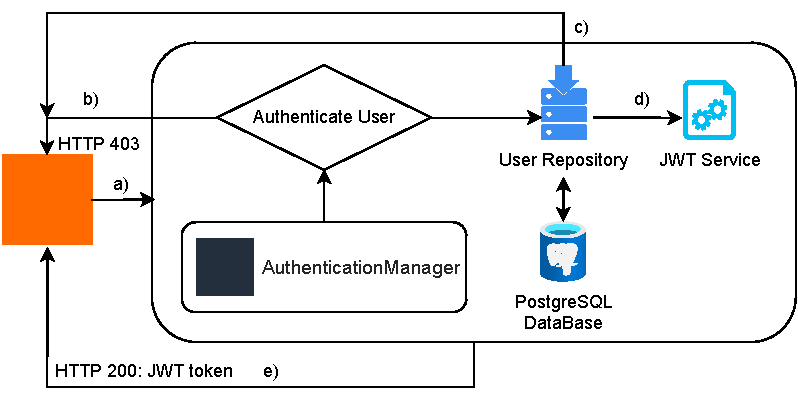
\includegraphics[scale=1.0]{rys03/proces_logowania}
    \caption{Schemat działania procesu logowania w systemie~\cite{JWToauth}}
    \label{fig:ebok_db_concept}
\end{figure}

Logowanie składa się z kilku kluczowych etapów:

\begin{enumerate}
    \item[\texttt{a)}] \textbf{Przesłanie danych logowania} -- Użytkownik wysyła żądanie HTTP \texttt{POST} na endpoint \texttt{/auth/login}, podając nazwę użytkownika oraz hasło. 

    \item[\texttt{b)}] \textbf{Weryfikacja przez \texttt{AuthenticationManager}} -- Spring Security wykorzystuje komponent \texttt{AuthenticationManager} do uwierzytelnienia użytkownika. Na tym etapie sprawdzana jest zgodność podanych danych logowania z zapisami w systemie.

    \item[\texttt{c)}] \textbf{Sprawdzenie w repozytorium użytkowników} -- \texttt{AuthenticationManager} deleguje żądanie do repozytorium użytkowników (\texttt{UserRepository}). Klasa \texttt{UserInfoManagerConfig}, implementująca interfejs \texttt{UserDetailsService}, sprawdza istnienie użytkownika w bazie danych i weryfikuje poprawność danych logowania. W~przypadku błędnych danych zwracany jest status \texttt{HTTP 403}.

    \item[\texttt{d)}] \textbf{Generowanie tokenu JWT} -- Po pomyślnym uwierzytelnieniu użytkownika generowany jest token JWT. Token zawiera informacje o użytkowniku (np.\ identyfikator, rolę oraz datę wygaśnięcia) i jest zabezpieczony przy użyciu kluczy RSA.

    \item[\texttt{e)}] \textbf{Przesłanie tokenu JWT w odpowiedzi} -- Token JWT jest zwracany użytkownikowi jako odpowiedź HTTP \texttt{200}. Jest przechowywany lokalnie (np.\ w pamięci przeglądarki) i~wykorzystywany do autoryzacji kolejnych żądań do API. Czas ważności tokenu wynosi 10 minut, co zapewnia równowagę między bezpieczeństwem a wygodą użytkownika.
\end{enumerate}

W szczególności klasa \texttt{UserInfoManagerConfig}, wykorzystywana w kroku \texttt{c)}, odpowiada za weryfikację istnienia użytkownika w bazie danych oraz dostarczenie szczegółów użytkownika wymaganych przez mechanizm uwierzytelniania. Kod klasy przedstawiono poniżej:

\begin{lstlisting}[language=Java, style=JavaStyle, caption=Klasa \texttt{UserInfoManagerConfig} odpowiedzialna za zarządzanie użytkownikami]
package bwp.hhn.backend.harmonyhomenetlogic.configuration.security;

import bwp.hhn.backend.harmonyhomenetlogic.repository.mainTables.UserRepository;
import lombok.RequiredArgsConstructor;
import org.springframework.security.core.userdetails.UserDetails;
import org.springframework.security.core.userdetails.UserDetailsService;
import org.springframework.security.core.userdetails.UsernameNotFoundException;
import org.springframework.stereotype.Service;

@Service
@RequiredArgsConstructor
public class UserInfoManagerConfig implements UserDetailsService {

    private final UserRepository userRepository;

    @Override
    public UserDetails loadUserByUsername(String username) throws UsernameNotFoundException {
        return userRepository.findByEmail(username)
                .orElseThrow(() -> new UsernameNotFoundException("User not found"));
    }
}
\end{lstlisting}

\noindent Kluczowe aspekty konfiguracji
Klasa \texttt{UserInfoManagerConfig}, używana podczas weryfikacji użytkownika, implementuje istotne elementy uwierzytelniania. Jej główne funkcje to:
\begin{itemize}
    \item \textbf{Weryfikacja użytkownika} -- Metoda \texttt{loadUserByUsername} sprawdza istnienie użytkownika w bazie danych na podstawie podanego adresu e-mail.
    \item \textbf{Obsługa błędów} -- W przypadku, gdy użytkownik nie zostanie znaleziony, zwracany jest wyjątek \texttt{UsernameNotFoundException}, kończący proces logowania.
    \item \textbf{Repozytorium użytkowników} -- Klasa korzysta z \texttt{UserRepository}, które zapewnia dostęp do bazy danych.
\end{itemize}

Mechanizm logowania w systemie jest bezpieczny i bezstanowy, co pozwala na ograniczenie ryzyka związanego z nieuprawnionym dostępem do zasobów oraz zwiększa wydajność. Dzięki zastosowaniu tokenów JWT proces uwierzytelniania jest szybki, a system nie wymaga utrzymywania sesji po stronie serwera, co upraszcza zarządzanie użytkownikami i zapewnia lepszą skalowalność.

\subsection{Zarządzanie tokenami JWT i autoryzacja użytkowników}

Zarządzanie tokenami JWT w systemie „Harmony Home Net” bazuje na mechanizmach walidacji i autoryzacji zaimplementowanych przy użyciu frameworka Spring Security. Proces ten zilustrowano na rysunku \ref{fig:resource_access_flow}. Jego główne etapy opisano poniżej.
\begin{figure}[ht]
    \centering
    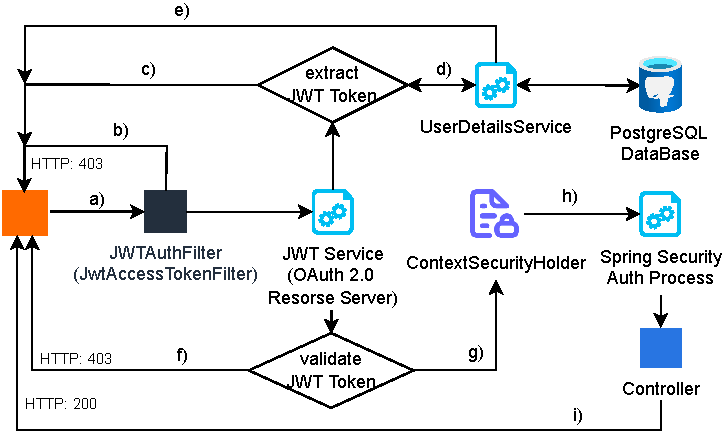
\includegraphics[scale=1]{rys03/Diagram_dotępu_do_zasobów_systemu} 
    \caption{Diagram zarządzania tokenami JWT i autoryzacji użytkowników~\cite{JWToauth}}
    \label{fig:resource_access_flow}
\end{figure}
\begin{enumerate}
    \item[\texttt{a)}] \textbf{Przesłanie żądania przez użytkownika} -- Użytkownik wysyła żądanie HTTP do serwera API, dołączając token JWT w nagłówku \texttt{Authorization}.
    
    \item[\texttt{b)}] \textbf{Przechwycenie żądania przez \texttt{JwtAccessTokenFilter}} -- Niestandardowy filtr \texttt{JwtAccessTokenFilter} przechwytuje żądanie i analizuje token JWT. Jeśli token jest niepoprawny lub nieobecny, użytkownik otrzymuje odpowiedź z kodem HTTP \texttt{403}.
    
    \item[\texttt{c)}] \textbf{Ekstrakcja danych z tokenu JWT} -- Token jest weryfikowany i dekodowany przez mechanizm \texttt{Jwt Service} w oparciu o \emph{OAuth 2.0 Resource Server}. Ekstrakcja danych, takich jak identyfikator użytkownika (\texttt{userEmail}), pozwala na kontynuację procesu autoryzacji. W przypadku błędów związanych z tokenem odpowiedź zawiera kod HTTP \texttt{403}.
    
    \item[\texttt{d)}] \textbf{Weryfikacja użytkownika w bazie danych} -- Wyodrębniony identyfikator użytkownika jest porównywany z danymi w bazie za pomocą \texttt{UserDetailsService}. Jeśli użytkownik nie istnieje w systemie, proces zostaje przerwany i zwracany jest kod HTTP \texttt{403}.
    
    \item[\texttt{e)}] \textbf{Walidacja tokenu JWT} -- Token JWT jest sprawdzany pod kątem poprawności oraz daty ważności. Jeśli token wygasł, odpowiedź zawiera kod HTTP \texttt{403}.
    
    \item[\texttt{f)}] \textbf{Tworzenie obiektu \texttt{UsernamePasswordAuthenticationToken}} -- W przypadku pomyślnej weryfikacji danych użytkownika tworzony jest obiekt \texttt{UsernamePasswordAuthenticationToken}, który przechowuje informacje o użytkowniku i jego uprawnieniach. Obiekt ten jest następnie zapisywany w \texttt{SecurityContextHolder}.
    
    \item[\texttt{g)}] \textbf{Autoryzacja zasobów} -- Spring Security sprawdza, czy użytkownik ma odpowiednie uprawnienia do żądanych zasobów. W przypadku braku odpowiednich uprawnień odpowiedź zawiera kod HTTP \texttt{403}.
    
    \item[\texttt{h)}] \textbf{Przekierowanie do kontrolera} -- Po pomyślnym uwierzytelnieniu żądanie jest przekazywane do kontrolera odpowiedzialnego za obsługę żądania.
    
    \item[\texttt{i)}] \textbf{Zwrócenie odpowiedzi} -- Kontroler zwraca odpowiedź JSON z kodem HTTP \texttt{200}, informując o sukcesie operacji.
\end{enumerate}

\noindent Kluczowe komponenty zarządzania tokenami JWT
Proces zarządzania tokenami opiera się na kilku kluczowych klasach:
\begin{itemize}
    \item \textbf{\texttt{JwtAccessTokenFilter}} -- Klasa odpowiedzialna za przechwytywanie żądań HTTP i analizę tokenów JWT. Filtr weryfikuje poprawność tokenu, sprawdza jego obecność na czarnej liście oraz zapisuje dane użytkownika w kontekście bezpieczeństwa.
    \item \textbf{\texttt{JwtTokenUtils}} -- Obsługuje operacje na tokenach JWT, takie jak ekstrakcja danych, sprawdzanie poprawności i walidacja zgodności z danymi użytkownika.
    \item \textbf{\texttt{JwtConfig}} -- Zapewnia konfigurację mechanizmów kodowania i dekodowania tokenów JWT przy użyciu kluczy RSA. Klucz publiczny służy do weryfikacji tokenu, natomiast klucz prywatny wykorzystywany jest podczas jego generowania.
\end{itemize}

\begin{lstlisting}[language=Java, style=JavaStyle, caption=Kod niestandardowego filtra \texttt{JwtAccessTokenFilter}]
@RequiredArgsConstructor
public class JwtAccessTokenFilter extends OncePerRequestFilter {

    private final RSAKeyRecord rsaKeyRecord;
    private final JwtTokenUtils jwtTokenUtils;
    private final TokenBlacklistService tokenBlacklistService;

    @Override
    protected void doFilterInternal(@NonNull HttpServletRequest request, 
                                    @NonNull HttpServletResponse response, 
                                    @NonNull FilterChain filterChain) 
            throws ServletException, IOException {

        final String authHeader = request.getHeader(HttpHeaders.AUTHORIZATION);

        if (authHeader == null || !authHeader.startsWith(TokenType.Bearer.name())) {
            filterChain.doFilter(request, response);
            return;
        }

        final String token = authHeader.substring(7);

        if (tokenBlacklistService.isTokenBlacklisted(token)) {
            response.setStatus(HttpStatus.UNAUTHORIZED.value());
            response.getWriter().write("Token is blacklisted");
            return;
        }

        JwtDecoder jwtDecoder = NimbusJwtDecoder.withPublicKey(rsaKeyRecord.publicKey()).build();
        Jwt jwtToken = jwtDecoder.decode(token);

        String userName = jwtTokenUtils.getUserName(jwtToken);

        if (userName != null && SecurityContextHolder.getContext().getAuthentication() == null) {
            UserDetails userDetails = jwtTokenUtils.userDetails(userName);

            if (jwtTokenUtils.isTokenValid(jwtToken, userDetails)) {
                UsernamePasswordAuthenticationToken authToken = new UsernamePasswordAuthenticationToken(
                        userDetails, null, userDetails.getAuthorities());
                authToken.setDetails(new WebAuthenticationDetailsSource().buildDetails(request));
                SecurityContextHolder.getContext().setAuthentication(authToken);
            }
        }
        filterChain.doFilter(request, response);
    }
}
\end{lstlisting}

\noindent Opis funkcji \texttt{JwtAccessTokenFilter}
\begin{itemize}
    \item Filtr przechwytuje każde żądanie HTTP i sprawdza obecność nagłówka \texttt{Authorization}.
    \item W razie złego tokenu lub jego braku użytkownik otrzymuje odpowiedź HTTP \texttt{403}.
    \item Token JWT jest dekodowany za pomocą klucza publicznego RSA, a jego dane są weryfikowane pod kątem zgodności z informacjami o użytkowniku.
    \item Po pomyślnej weryfikacji dane użytkownika są zapisywane w kontekście bezpieczeństwa, umożliwiając dalszy proces autoryzacji.
\end{itemize}

\begin{lstlisting}[language=Java, style=JavaStyle, caption=Klasa \texttt{JwtConfig}]
@Configuration
public class JwtConfig {

    private final RSAKeyRecord rsaKeyRecord;

    public JwtConfig(RSAKeyRecord rsaKeyRecord) {
        this.rsaKeyRecord = rsaKeyRecord;
    }

    @Bean
    public JwtDecoder jwtDecoder() {
        return NimbusJwtDecoder.withPublicKey(rsaKeyRecord.publicKey()).build();
    }

    @Bean
    public JwtEncoder jwtEncoder() {
        JWK jwk = new RSAKey.Builder(rsaKeyRecord.publicKey())
                           .privateKey(rsaKeyRecord.privateKey())
                           .build();
        JWKSource<SecurityContext> jwkSource = new ImmutableJWKSet<>(new JWKSet(jwk));
        return new NimbusJwtEncoder(jwkSource);
    }
}
\end{lstlisting}

\begin{lstlisting}[language=Java, style=JavaStyle, caption=Klasa \texttt{JwtTokenUtils}]
@Component
@RequiredArgsConstructor
public class JwtTokenUtils {

    private final UserRepository userRepository;

    public String getUserName(Jwt jwtToken) {
        return jwtToken.getSubject();
    }

    public boolean isTokenValid(Jwt jwtToken, UserDetails userDetails) {
        final String userName = getUserName(jwtToken);
        boolean isTokenExpired = jwtToken.getExpiresAt().isBefore(Instant.now());
        return !isTokenExpired && userName.equals(userDetails.getUsername());
    }

    public UserDetails userDetails(String email) {
        return userRepository.findByEmail(email)
                .orElseThrow(() -> new UsernameNotFoundException("User not found"));
    }
}
\end{lstlisting}


\subsection{Zarządzanie czarną listą tokenów}

Mechanizm zarządzania czarną listą tokenów w systemie „Harmony Home Net” zapewnia możliwość unieważnienia tokenów JWT, co jest kluczowe podczas wylogowywania użytkowników. Dzięki temu rozwiązaniu system natychmiast kończy sesję użytkownika, uniemożliwiając dalszy dostęp do chronionych zasobów przy użyciu unieważnionego tokenu.\\[-10pt]

\noindent \textbf{Proces wylogowania i dodawania tokenu do czarnej listy}\newline
Wylogowanie użytkownika odbywa się za pomocą specjalnego łańcucha filtrów \texttt{logoutSecurityFilterChain}, zdefiniowanego w klasie \texttt{SecurityConfig}. Kod konfiguracji łańcucha wylogowania przedstawiono poniżej.

\begin{lstlisting}[language=Java, style=JavaStyle, caption=Konfiguracja łańcucha wylogowania]
@Bean
@Order(4)
public SecurityFilterChain logoutSecurityFilterChain(HttpSecurity httpSecurity) throws Exception {
    return httpSecurity
            .securityMatcher(new AntPathRequestMatcher("/logout"))
            .csrf(AbstractHttpConfigurer::disable)
            .authorizeHttpRequests(auth -> auth.anyRequest().authenticated())
            .oauth2ResourceServer(oauth2 -> oauth2.jwt(withDefaults()))
            .sessionManagement(session -> session.sessionCreationPolicy(SessionCreationPolicy.STATELESS))
            .logout(logout -> logout
                    .logoutUrl("/logout")
                    .logoutSuccessHandler((request, response, authentication) -> {
                        String token = request.getHeader("Authorization").replace("Bearer ", "");
                        tokenBlacklistService.blacklistToken(token);
                        SecurityContextHolder.clearContext();
                    })
            )
            .cors(withDefaults())
            .build();
}
\end{lstlisting}

\noindent W procesie wylogowania system wykonuje następujące kroki:
\begin{itemize}
    \item Ekstrakcja tokenu JWT z nagłówka \texttt{Authorization}.
    \item Dodanie tokenu do czarnej listy za pomocą \texttt{TokenBlacklistService}.
    \item Wyczyszczenie kontekstu bezpieczeństwa (\texttt{SecurityContextHolder}), co skutkuje natychmiastowym unieważnieniem sesji użytkownika.
\end{itemize}

\noindent \textbf{Zarządzanie czarną listą tokenów}\newline
Za przechowywanie i obsługę czarnej listy tokenów odpowiada klasa \texttt{TokenBlacklistService}. Kod tej klasy przedstawiono poniżej.

\begin{lstlisting}[language=Java, style=JavaStyle, caption=Klasa \texttt{TokenBlacklistService}]
@Service
@RequiredArgsConstructor
public class TokenBlacklistService {
    private final Set<String> blacklistedTokens = new HashSet<>();
    private final JwtDecoder jwtDecoder;

    public void blacklistToken(String token) {
        blacklistedTokens.add(token);
    }

    public boolean isTokenBlacklisted(String token) {
        return blacklistedTokens.contains(token);
    }

    @Scheduled(cron = "0 */15 * * * *") // Every 15 minutes
    @Async
    public void clearExpiredTokens() {
        blacklistedTokens.removeIf(this::isTokenExpired);
    }

    private boolean isTokenExpired(String token) {
        return Date.from(
                Objects.requireNonNull(
                        jwtDecoder.decode(token).getExpiresAt()
                )
        ).before(new Date());
    }
}
\end{lstlisting}

\noindent Funkcje klasy \texttt{TokenBlacklistService}:
\begin{itemize}
    \item \texttt{blacklistToken} -- dodaje token JWT do czarnej listy, co uniemożliwia jego dalsze wykorzystanie.
    \item \texttt{isTokenBlacklisted} -- sprawdza, czy dany token znajduje się na czarnej liście.
    \item \texttt{clearExpiredTokens} -- usuwa wygasłe tokeny z czarnej listy, co zwalnia pamięć.
\end{itemize}

\noindent \textbf{Harmonogram czyszczenia czarnej listy}\newline
Usługa \texttt{TokenBlacklistService} korzysta z harmonogramowanego zadania (\texttt{@Scheduled}), które co 15 minut przeszukuje czarną listę i usuwa tokeny, które wygasły. Operacja ta jest realizowana asynchronicznie, co zapobiega wpływowi na wydajność systemu.

Mechanizm czarnej listy tokenów pozwala skutecznie zabezpieczyć system przed dostępem nieautoryzowanym po wylogowaniu użytkownika lub w przypadku naruszeń bezpieczeństwa.


\subsection{Mechanizmy resetowania hasła}

Mechanizm resetowania hasła zaprojektowano z uwzględnieniem podstawowych zasad bezpieczeństwa, jednak w uproszczonej formie w stosunku do pełnoprawnych wdrożeń produkcyjnych. Na interfejsie użytkownika uwidacznia się to jak na rysunku~\ref{fig:ui_password_reset}.
\begin{figure}[ht]
    \centering
    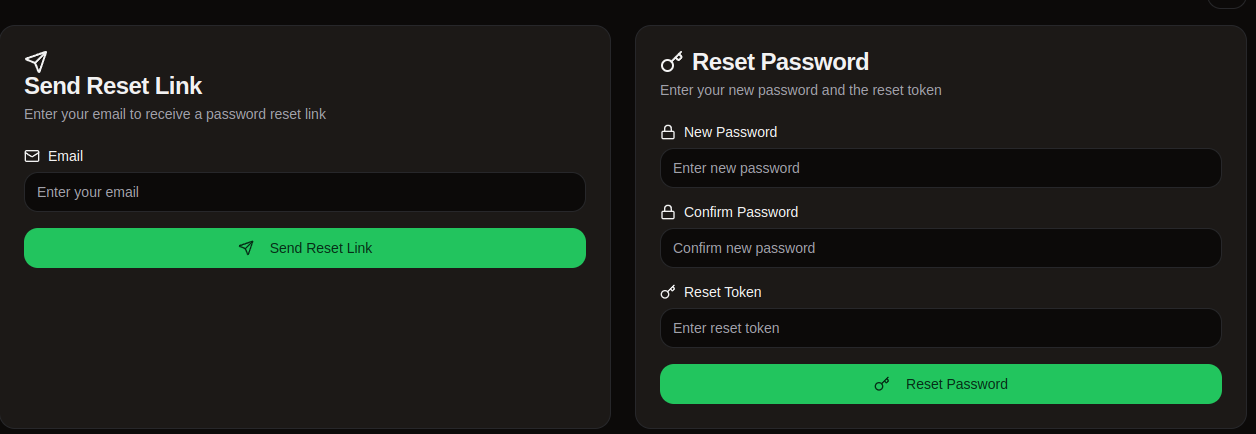
\includegraphics[width=0.95\linewidth]{rys03/pass_resert}
    \caption{Interfejs użytkownika wykorzystywany podczas resetowania}
    \label{fig:ui_password_reset}
\end{figure}

\noindent Resetowanie hasła przebiega według następujących kroków:
\begin{itemize}
    \item \textbf{Prośba o reset hasła} -- użytkownik wprowadza swój adres e-mail w sekcji \emph{Send Reset Link} i przesyła żądanie na endpoint \texttt{/forgot-password}. Na wskazany adres e-mail wysyłany jest unikalny token resetujący.
    
    \item \textbf{Resetowanie hasła} -- w sekcji \emph{Reset Password} użytkownik wprowadza nowe hasło, jego potwierdzenie oraz token resetujący. Formularz przesyła dane na endpoint \texttt{/reset-password}, który weryfikuje token, sprawdza jego ważność i aktualizuje hasło w bazie danych.
    
    \item \textbf{Bezpieczeństwo} -- tokeny resetujące są jednorazowe i mają ograniczony czas ważności. System wymusza także spełnienie kryteriów bezpieczeństwa dla nowych haseł.
    
    \item \textbf{Zmiana hasła} -- dla zalogowanych użytkowników dostępny jest dedykowany endpoint \texttt{/change-password}, który umożliwia zmianę hasła bez konieczności resetowania. Funkcjonalność ta znajduje się w zakładce \textbf{Ustawienia} w panelu użytkownika.
\end{itemize}

Mechanizm został zaimplementowany w kontrolerze \texttt{AuthController}, który obsługuje odpowiednie endpointy. Kod przedstawiono poniżej.

\begin{lstlisting}[language=Java, style=JavaStyle, caption=Fragment klasy \texttt{AuthController}]
@PostMapping("/forgot-password")
public ResponseEntity<String> forgotPassword(@RequestBody PasswordResetRequest request) {
    authService.forgotPassword(request.getEmail());
    return ResponseEntity.ok("Password reset link has been sent to your email.");
}

@PostMapping("/reset-password")
public ResponseEntity<String> resetPassword(@RequestBody PasswordUpdateRequest request) {
    authService.resetPassword(request.getToken(), request.getNewPassword(), request.getConfirmPassword());
    return ResponseEntity.ok("Password has been reset successfully.");
}

@PostMapping("/change-password")
public ResponseEntity<String> changePassword(@RequestBody PasswordChangeRequest request) {
    authService.changePassword(request.getNewPassword(), request.getConfirmPassword(), request.getEmail());
    return ResponseEntity.ok("Password has been changed successfully.");
}
\end{lstlisting}

Znaczenie poszczególnych endpointów:
\begin{itemize}
    \item \texttt{forgotPassword} -- generuje jednorazowy token resetujący i wysyła go na adres e-mail użytkownika.
    \item \texttt{resetPassword} -- weryfikuje token oraz zgodność przesłanych haseł. W przypadku poprawnej walidacji aktualizuje hasło użytkownika w bazie danych.
    \item \texttt{changePassword} -- umożliwia zalogowanym użytkownikom zmianę hasła po podaniu aktualnych danych.
\end{itemize}

Proces resetowania hasła obsługiwany jest przez klasę \texttt{AuthServiceImp}, implementującą interfejs \texttt{AuthService}. Kluczowe metody przedstawiono poniżej.

\begin{lstlisting}[language=Java, style=JavaStyle, caption=Metody resetowania hasła w klasie \texttt{AuthServiceImp}]
@Override
public void forgotPassword(String email) {
    User user = userRepository.findByEmail(email)
            .orElseThrow(() -> new UserNotFoundException("User not found"));

    String token = bCryptPasswordEncoder.encode(UUID.randomUUID().toString());
    user.setResetToken(token);
    user.setResetTokenExpiry(Instant.now().plus(1, ChronoUnit.HOURS));
    userRepository.save(user);

    mailService.sendNotificationMail(
            "Password Reset Request",
            token,
            user.getEmail()
    );
}

@Override
public void resetPassword(String token, String newPassword, String confirmPassword) {
    User user = userRepository.findByResetToken(token)
            .orElseThrow(() -> new ResponseStatusException(HttpStatus.BAD_REQUEST, "Invalid token"));

    if (!newPassword.equals(confirmPassword)) {
        throw new ResponseStatusException(HttpStatus.BAD_REQUEST, "Passwords do not match");
    }

    if (user.getResetTokenExpiry().isBefore(Instant.now())) {
        throw new ResponseStatusException(HttpStatus.BAD_REQUEST, "Token has expired");
    }

    user.setPassword(bCryptPasswordEncoder.encode(newPassword));
    user.setResetToken(null);
    user.setResetTokenExpiry(null);
    userRepository.save(user);
}
\end{lstlisting}

\noindent Działanie metod:
\begin{itemize}
    \item \texttt{forgotPassword} -- generuje token resetujący, ustawia jego czas ważności i wysyła e-mail z~instrukcjami.
    \item \texttt{resetPassword} -- weryfikuje token, sprawdza zgodność nowego hasła z potwierdzeniem i~aktualizuje dane użytkownika w bazie.
\end{itemize}

%%\noindent \textbf{Bezpieczeństwo i rozwój}\newline
\noindent Obecna implementacja zapewnia podstawowe mechanizmy ochrony:
\begin{enumerate}
    \item Tokeny są jednorazowe, szyfrowane i mają ograniczony czas ważności.
    \item Nowe hasła muszą spełniać wymagania dotyczące bezpieczeństwa.
    \item Weryfikacja zgodności haseł minimalizuje ryzyko błędów użytkownika.
\end{enumerate}
W przyszłości system może zostać rozbudowany o:
\begin{itemize}
    \item Audyt operacji resetowania hasła.
    \item Wdrożenie wieloskładnikowego uwierzytelniania (MFA) podczas resetu.
    \item Wysyłanie linku resetującego zamiast tokenu w treści e-maila.
\end{itemize}

Mechanizm resetowania hasła, mimo uproszczeń w prototypie, spełnia kluczowe wymagania bezpieczeństwa i może być łatwo rozszerzony w przyszłych wersjach systemu.

\section{Zarządzanie użytkownikami}

System zarządzania użytkownikami w prototypie „Harmony Home Net” został zaprojektowany jako zamknięty system, co oznacza, że rejestracja nowych użytkowników odbywa się wyłącznie za pośrednictwem pracowników administracyjnych. Takie podejście pozwala zwiększyć bezpieczeństwo, ograniczając dostęp do systemu jedynie do osób upoważnionych.

\subsection{Encja użytkownika \texttt{User}}

Encja \texttt{User} stanowi jeden z kluczowych elementów systemu zarządzania użytkownikami. Reprezentuje dane użytkownika, takie jak imię, nazwisko, adres e-mail, numer telefonu oraz przypisana rola. Klasa ta implementuje interfejs \texttt{UserDetails} z biblioteki Spring Security, co umożliwia jej bezpośrednie wykorzystanie w procesach uwierzytelniania i autoryzacji. Najważniejsze cechy encji \texttt{User} to:
\begin{itemize}
    \item \textbf{Integracja z mechanizmami Spring Security} -- implementacja interfejsu \texttt{UserDetails} umożliwia przechowywanie danych uwierzytelniających i ich wykorzystanie w procesach autoryzacji.
    \item \textbf{Adnotacje JPA} -- klasa jest zmapowana na tabelę \texttt{Users} w bazie danych za pomocą adnotacji takich jak \texttt{@Entity}, \texttt{@Table} oraz \texttt{@Column}.
    \item \textbf{Relacje z innymi encjami} -- encja posiada powiązania z tabelami, takimi jak \texttt{NotificationType}, \texttt{UserDocumentConnection} oraz \texttt{PossessionHistory}, co odzwierciedla jej rolę w systemie.
    \item \textbf{Bezpieczeństwo danych} -- hasła użytkowników są walidowane i szyfrowane przed zapisem do bazy danych, zapewniając ochronę wrażliwych informacji.
\end{itemize}

Poniżej przedstawiono kod encji \texttt{User}.
\begin{lstlisting}[language=Java, style=JavaStyle, caption=Encja użytkownika \texttt{User}]
@Data
@AllArgsConstructor
@NoArgsConstructor
@Builder
@Entity
@Table(name = "Users", indexes = {
	@Index(name = "idx_user_email_unq", columnList = "Email", unique = true),
	@Index(name = "idx_user_uuid", columnList = "UUID_id", unique = true)
})
public class User implements UserDetails {

    @Id
    @GeneratedValue(strategy = GenerationType.UUID)
    @Column(name = "UUID_id")
    private UUID uuidID;

    @NotEmpty
    @Size(min = 3, max = 50)
    @Column(name = "First_name", nullable = false, length = 50)
    private String firstName;

    @NotEmpty
    @Size(min = 3, max = 50)
    @Column(name = "Last_name", nullable = false, length = 50)
    private String lastName;

    @NotEmpty
    @Email
    @Pattern(regexp = "^[A-Za-z0-9+_.-]+@(.+)$", message = "Invalid email format")
    @Column(name = "Email", nullable = false, unique = true, length = 50)
    private String email;

    @NotEmpty
    @Size(min = 10, max = 255)
    @Column(name = "Password", nullable = false)
    private String password;

    @Column(name = "Role", length = 20)
    @Enumerated(EnumType.STRING)
    private Role role;

    @NotEmpty
    @Pattern(regexp = "^\\d{9,11}$", message = "Invalid phone number format")
    @Column(name = "Phone_number", nullable = false, unique = true, length = 11)
    private String phoneNumber;

    @CreationTimestamp
    @Column(name = "Create_at")
    private Instant createdAt;

    @UpdateTimestamp
    @Column(name = "Update_at")
    private Instant updatedAt;

    @OneToMany(mappedBy = "user", cascade = CascadeType.ALL, orphanRemoval = true)
    @JsonManagedReference
    private List<NotificationType> notificationTypes;

    @OneToMany(mappedBy = "user", cascade = CascadeType.ALL, orphanRemoval = true)
    @JsonManagedReference
    private List<UserDocumentConnection> userDocumentConnections;

    @Column(name = "reset_token")
    private String resetToken;

    @Column(name = "reset_token_expiry")
    private Instant resetTokenExpiry;

    @Override
    public Collection<? extends GrantedAuthority> getAuthorities() {
        return List.of(role);
    }

    @Override
    public String getPassword() {
        return password;
    }

    @Override
    public String getUsername() {
        return email;
    }
}
\end{lstlisting}

\noindent \textbf{Rola w autoryzacji użytkowników} -- dzięki metodzie \texttt{getAuthorities()} encja umożliwia odczytywanie ról przypisanych użytkownikowi. W połączeniu z mechanizmami Spring Security pozwala to na efektywne zarządzanie dostępem do zasobów systemu.

\subsection{Role i poziomy dostępu}

System zarządzania użytkownikami opiera się na hierarchii ról definiujących poziom uprawnień. Klasa \texttt{Role} pozwala określić, czy użytkownik ma wystarczające uprawnienia do wykonania określonych operacji, jak edycja danych innych użytkowników czy przypisanie nowej roli. Dostępne role:
\begin{itemize}
    \item \texttt{ROLE\_OWNER} -- poziom 1, właściciel mieszkania, podstawowa rola w systemie.
    \item \texttt{ROLE\_EMPLOYEE} -- poziom 2, pracownik administracyjny.
    \item \texttt{ROLE\_ADMIN} -- poziom 3, administrator systemu.
    \item \texttt{ROLE\_SUPER\_ADMIN} -- poziom 4, superadministrator, najwyższy poziom dostępu.
\end{itemize}

\noindent \textbf{Zasady działania hierarchii ról}:
\begin{itemize}
    \item Każda rola ma przypisaną wartość \texttt{level}, określającą jej miejsce w hierarchii.
    \item Operacje takie jak przypisanie nowej roli są dozwolone wyłącznie dla użytkowników posiadających wyższy poziom \texttt{level} niż modyfikowany użytkownik.
    \item Rola \texttt{ROLE\_OWNER} jest dodatkowo zabezpieczona przed zmianami, co wymusza usunięcie i ponowną rejestrację użytkownika w celu zmiany jego uprawnień.
\end{itemize}

\noindent Poniżej przedstawiono kod definiujący hierarchię ról.
\begin{lstlisting}[language=Java, style=JavaStyle, caption=Definicja ról w systemie \texttt{Role}]
package bwp.hhn.backend.harmonyhomenetlogic.utils.enums;

import lombok.Getter;
import org.springframework.security.core.GrantedAuthority;

@Getter
public enum Role implements GrantedAuthority {
    ROLE_OWNER(1), ROLE_EMPLOYEE(2), ROLE_ADMIN(3), ROLE_SUPER_ADMIN(4);

    private final int level;

    Role(int level) {
        this.level = level;
    }

    @Override
    public String getAuthority() {
        return name();
    }
}
\end{lstlisting}

\subsection{Dodawanie użytkowników i przypisywanie ról}

Proces zarządzania użytkownikami, obejmujący ich dodawanie i edycję, opiera się na mechanizmie autoryzacji bazującym na poziomach dostępu przypisanych do ról w enumeracji \texttt{Role}. Każda rola (\texttt{ROLE\_OWNER}, \texttt{ROLE\_EMPLOYEE}, \texttt{ROLE\_ADMIN}, \texttt{ROLE\_SUPER\_ADMIN}) ma określony poziom dostępu, co pozwala kontrolować uprawnienia do wykonywania operacji takich jak dodawanie, edycja czy usuwanie użytkowników.\\[-10pt]

\textbf{Kluczowe założenia mechanizmu:}
\begin{itemize}
    \item \textbf{Hierarchia poziomów dostępu} -- wartości liczbowe przypisane do ról zapewniają, że użytkownicy z wyższymi poziomami uprawnień mogą zarządzać użytkownikami posiadającymi role o niższym poziomie.
    \item \textbf{Zabezpieczenie ról} -- rola \texttt{ROLE\_OWNER} jest szczególnie chroniona i nie może być zmieniona bez usunięcia użytkownika i jego ponownej rejestracji z nową rolą.
\end{itemize}

Proces rejestracji użytkownika został zaimplementowany w usłudze \texttt{AuthServiceImp}. Kluczowe elementy tego procesu to:
\begin{itemize}
    \item \textbf{Weryfikacja uprawnień pracownika rejestrującego} -- token JWT dostarczony przez pracownika jest weryfikowany, aby upewnić się, że osoba wykonująca operację ma odpowiednie uprawnienia.
    \item \textbf{Przypisywanie ról} -- nowym użytkownikom można przypisać jedną z dostępnych ról. Mechanizm weryfikuje, czy osoba rejestrująca ma wystarczające uprawnienia do przypisania danej roli.
    \item \textbf{Wysyłanie e-maila powitalnego} -- po pomyślnej rejestracji użytkownik otrzymuje e-mail z~informacją o utworzeniu konta.
\end{itemize}

\noindent Poniżej przedstawiono fragment kodu obsługującego rejestrację użytkownika.
\begin{lstlisting}[language=Java, style=JavaStyle, caption=Rejestracja użytkownika w \texttt{AuthServiceImp}]
@Override
@Transactional
public String register(RegisterRequest userRequest, String accessToken) {
    JwtDecoder jwtDecoder = NimbusJwtDecoder.withPublicKey(rsaKeyRecord.publicKey()).build();
    final Jwt jwtToken = jwtDecoder.decode(accessToken);

    Role role = Role.valueOf(jwtToken.getClaim("role"));

    if (role.getLevel() < userRequest.getRole().getLevel()) {
        throw new ResponseStatusException(HttpStatus.UNAUTHORIZED, "Insufficient permissions to update or assign the role");
    }

    if (userRepository.existsByEmail(userRequest.getEmail())) {
        throw new ResponseStatusException(HttpStatus.CONFLICT, "Email already exists");
    }

    User user = User.builder()
            .email(userRequest.getEmail())
            .password(bCryptPasswordEncoder.encode(userRequest.getPassword()))
            .role(userRequest.getRole())
            .firstName(userRequest.getFirstName())
            .lastName(userRequest.getLastName())
            .phoneNumber(userRequest.getPhoneNumber())
            .build();

    userRepository.save(user);
    mailService.sendNotificationMail("Welcome to Harmony Home Net", "Your account has been successfully created.", user.getEmail());
    return "User registered successfully.";
}
\end{lstlisting}

\subsection{Zarządzanie użytkownikami i ich danymi}

System zarządzania użytkownikami zapewnia funkcje takie jak:
\begin{itemize}
    \item \textbf{Paginacja} -- stronicowanie umożliwia efektywne zarządzanie dużą liczbą użytkowników.
    \item \textbf{Edycja danych użytkownika} -- administratorzy mogą zmieniać dane użytkowników, w tym e-mail, imię, nazwisko oraz przypisaną rolę.
    \item \textbf{Usuwanie użytkowników} -- system pozwala na usuwanie użytkowników wraz z powiązanymi danymi, np. powiadomieniami czy historią posiadania nieruchomości.
\end{itemize}

\noindent Poniżej przedstawiono fragment kodu obsługującego edycję użytkownika.
\begin{lstlisting}[language=Java, style=JavaStyle, caption=Edycja użytkownika w \texttt{UserServiceImp}]
@Override
public UserResponse updateUser(UUID userId, UserRequest user, String accessToken) throws UserNotFoundException {
    JwtDecoder jwtDecoder = NimbusJwtDecoder.withPublicKey(rsaKeyRecord.publicKey()).build();
    final Jwt jwtToken = jwtDecoder.decode(accessToken);

    Role role = Role.valueOf(jwtToken.getClaim("role"));

    if (role.getLevel() < user.getRole().getLevel()) {
        throw new ResponseStatusException(HttpStatus.UNAUTHORIZED, "Insufficient permissions to update or assign the role");
    }

    User userEntity = userRepository.findByUuidIDOrEmail(userId, null)
            .orElseThrow(() -> new UserNotFoundException("User id: " + userId + " not found"));

    if (userEntity.getRole() == Role.ROLE_OWNER && user.getRole() != Role.ROLE_OWNER) {
        throw new ResponseStatusException(HttpStatus.UNAUTHORIZED, "Cannot change the role of an OWNER");
    }

    if ((userEntity.getRole() == Role.ROLE_ADMIN || userEntity.getRole() == Role.ROLE_EMPLOYEE) && user.getRole() == Role.ROLE_OWNER) {
        throw new ResponseStatusException(HttpStatus.UNAUTHORIZED, "Cannot change the role to OWNER");
    }

    userEntity.setEmail(user.getEmail() != null ? user.getEmail() : userEntity.getEmail());
    userEntity.setFirstName(user.getFirstName() != null ? user.getFirstName() : userEntity.getFirstName());
    userEntity.setLastName(user.getLastName() != null ? user.getLastName() : userEntity.getLastName());
    userEntity.setPhoneNumber(user.getPhoneNumber() != null ? user.getPhoneNumber() : userEntity.getPhoneNumber());
    userEntity.setRole(user.getRole() != null ? user.getRole() : userEntity.getRole());
    userEntity.setPassword(user.getPassword() != null ? bCryptPasswordEncoder.encode(user.getPassword()) : userEntity.getPassword());

    User saved = userRepository.save(userEntity);

    return UserResponse.builder()
            .email(saved.getEmail())
            .firstName(saved.getFirstName())
            .lastName(saved.getLastName())
            .updatedAt(saved.getUpdatedAt())
            .createdAt(saved.getCreatedAt())
            .phoneNumber(saved.getPhoneNumber())
            .build();
}
\end{lstlisting}

\noindent Poniżej przedstawiono fragment kontrolera odpowiedzialnego za paginację i zarządzanie użytkownikami.
\begin{lstlisting}[language=Java, style=JavaStyle, caption=Metoda paginacji w \texttt{UserController}]
@GetMapping("/get-all-users")
public ResponseEntity<PageResponse<UserResponse>> getAllUsers(
        @RequestParam(value = "pageNo", defaultValue = "0", required = false) int pageNo,
        @RequestParam(value = "pageSize", defaultValue = "10", required = false) int pageSize) {
    return ResponseEntity.ok(userService.getAllUsers(pageNo, pageSize));
}
\end{lstlisting}

\subsection{Potencjalna integracja ACL}

W ramach rozwoju systemu rozważana jest integracja mechanizmu \textbf{ACL}~\cite{acl}, umożliwiającego precyzyjne zarządzanie dostępem do zasobów. Mechanizm ten pozwala przypisywać uprawnienia na poziomie poszczególnych obiektów, np. ograniczając dostęp użytkowników do wybranych zgłoszeń technicznych.

\noindent Możliwe zastosowania ACL:
\begin{itemize}
    \item Definiowanie uprawnień na poziomie obiektów, jak mieszkania czy zgłoszenia techniczne.
    \item Hierarchiczne zarządzanie uprawnieniami, stosowne do struktury wspólnoty mieszkaniowej.
    \item Audyt i logowanie działań użytkowników, co pozwala monitorować potencjalne nadużycia.
\end{itemize}

Obecnie zarządzanie użytkownikami i przypisywanie ról w systemie stanowi solidny fundament, który w przyszłości może zostać rozwinięty o bardziej zaawansowane mechanizmy takie jak ACL.

\section{Zarządzanie mieszkaniami}

Zarządzanie mieszkaniami w prototypie systemu ,,Harmony Home Net'' jest kluczowym elementem jego funkcjonalności. Mieszkanie stanowi jedną z dwóch podstawowych tabel w systemie, obok tabeli użytkowników. W tej sekcji opisano strukturę encji \texttt{Apartment}, tabelę pośredniczącą \texttt{PossessionHistory}, mechanizmy przypisywania właścicieli oraz możliwe kierunki rozwoju tego modułu.

\subsection{Encja \texttt{Apartment}}

Encja \texttt{Apartment} reprezentuje mieszkanie w systemie i przechowuje kluczowe informacje, takie jak adres, powierzchnia, wartość procentowa oraz unikalna sygnatura. Struktura encji została zaprojektowana w sposób umożliwiający łatwe zarządzanie danymi oraz integrację z innymi elementami systemu.

\begin{itemize}
    \item \textbf{Adres i lokalizacja} -- Każde mieszkanie posiada informacje o adresie, mieście oraz kodzie pocztowym, które są walidowane podczas dodawania.
    \item \textbf{Powierzchnia i wartość procentowa} -- Dane dotyczące powierzchni mieszkania i jego udziału procentowego w całej wspólnocie są przechowywane z wysoką precyzją dzięki typowi \texttt{BigDecimal}.
    \item \textbf{Relacje} -- Encja posiada relację z tabelą \texttt{PossessionHistory}, umożliwiającą przypisywanie mieszkań do użytkowników i zarządzanie historią posiadania.
\end{itemize}

\noindent Poniżej przedstawiono fragment kodu encji \texttt{Apartment}.

\begin{lstlisting}[language=Java, style=JavaStyle, caption=Encja mieszkania \texttt{Apartment}]
@Data
@AllArgsConstructor
@NoArgsConstructor
@Builder
@Entity
@Table(name = "Apartments", indexes = {
        @Index(name = "idx_apartment_unq", columnList = "Apartment_signature", unique = true)
})
public class Apartment {

    @Id
    @GeneratedValue(strategy = GenerationType.UUID)
    @Column(name = "UUID_id")
    private UUID uuidID;

    @NotNull
    @Size(min = 1, max = 60)
    @Column(name = "Apartment_signature", nullable = false, unique = true, length = 60)
    private String apartmentSignature;

    @NotEmpty
    @Size(max = 50)
    @Column(name = "Address", nullable = false, length = 50)
    private String address;

    @NotEmpty
    @Size(max = 20)
    @Column(name = "City", nullable = false, length = 20)
    private String city;

    @NotEmpty
    @Pattern(regexp = "^\\d{2}-\\d{3}$", message = "Invalid zip code format")
    @Column(name = "Zip_code", nullable = false, length = 6)
    private String zipCode;

    @NotNull
    @DecimalMin(value = "0.0", inclusive = false)
    @Digits(integer = 3, fraction = 2)
    @Column(name = "Apartment_area", nullable = false, precision = 5, scale = 2)
    private BigDecimal apartmentArea;

    @NotNull
    @DecimalMin(value = "0.0", inclusive = false)
    @Column(name = "Apartment_percent_value", nullable = false, precision = 5, scale = 2)
    private BigDecimal apartmentPercentValue;

    @CreationTimestamp
    @Column(name = "Create_at", nullable = false, updatable = false)
    private Instant createdAt;

    @UpdateTimestamp
    @Column(name = "Update_at", updatable = false)
    private Instant updatedAt;

    @OneToMany(mappedBy = "apartment", cascade = CascadeType.ALL, orphanRemoval = true)
    private List<PossessionHistory> possessionHistories;

    // Additional relationships and fields
}
\end{lstlisting}

\subsection{Tabela pośrednicząca \texttt{PossessionHistory}}

Tabela \texttt{PossessionHistory} pełni rolę pośredniczącą między użytkownikami a mieszkaniami. Pozwala zarządzać przypisaniami oraz przechowywać historię posiadania. Każdy związek użytkownik-mieszkanie jest unikalny, co zapewnia integralność danych.

\begin{itemize}
    \item \textbf{Historia przypisań} -- Każdy rekord przechowuje daty rozpoczęcia i zakończenia posiadania mieszkania.
    \item \textbf{Dodatkowe informacje} -- Możliwość przechowywania notatek związanych ze statusem przypisania.
    \item \textbf{Relacje} -- Tabela jest połączona zarówno z tabelą użytkowników, jak i mieszkań.
\end{itemize}

Fragment kodu tabeli \texttt{PossessionHistory}:

\begin{lstlisting}[language=Java, style=JavaStyle, caption=Tabela pośrednicząca \texttt{PossessionHistory}]
@Data
@AllArgsConstructor
@NoArgsConstructor
@Builder
@Entity
@Table(name = "Possession_history", indexes = {
        @Index(name = "idx_possession_user_id", columnList = "user_id"),
        @Index(name = "idx_possession_apartment_id", columnList = "apartment_id"),
        @Index(name = "idx_possession_start_date", columnList = "start_date"),
        @Index(name = "idx_possession_end_date", columnList = "end_date")
}, uniqueConstraints = {
        @UniqueConstraint(columnNames = {"user_id", "apartment_id"})
})
public class PossessionHistory {

    @Id
    @GeneratedValue(strategy = GenerationType.IDENTITY)
    @Column(name = "ID")
    private Long id;

    @CreationTimestamp
    @Column(name = "Start_date", nullable = false)
    private Instant startDate;

    @Column(name = "End_date")
    private Instant endDate;

    @Column(name = "Status_notes", length = 1000)
    private String statusNotes;

    @ManyToOne
    @JoinColumn(name = "user_id", referencedColumnName = "UUID_id")
    private User user;

    @ManyToOne
    @JoinColumn(name = "apartment_id", referencedColumnName = "UUID_id")
    private Apartment apartment;
}
\end{lstlisting}

\subsection{Przypisywanie i odłączanie właścicieli}

Proces przypisywania mieszkania do użytkownika jest realizowany w serwisie \texttt{ApartmentsServiceImp}. W trakcie przypisywania sprawdzane są następujące aspekty:
\begin{itemize}
    \item \textbf{Istnienie użytkownika i mieszkania} -- Weryfikacja obecności użytkownika i mieszkania w~systemie.
    \item \textbf{Unikalność przypisania} -- Sprawdzenie, czy użytkownik nie ma już przypisanego danego mieszkania.
\end{itemize}

\noindent Poniżej przedstawiono fragment implementacji przypisywania właścicieli.

\begin{lstlisting}[language=Java, style=JavaStyle, caption=Przypisywanie właścicieli w \texttt{ApartmentsServiceImp}]
@Override
@Transactional
public PossessionHistoryResponse createPossessionHistory(String apartmentSignature, UUID userId)
        throws ApartmentNotFoundException, UserNotFoundException {
    User user = userRepository.findById(userId)
            .orElseThrow(() -> new UserNotFoundException("User: " + userId + " not found"));

    Apartment apartment = apartmentsRepository.findByApartmentSignature(apartmentSignature)
            .orElseThrow(() -> new ApartmentNotFoundException("Apartment with signature: " + apartmentSignature + " not found"));

    if (possessionHistoryRepository.existsByUserUuidIDAndApartmentUuidID(userId, apartment.getUuidID())) {
        throw new ApartmentNotFoundException("User already has this apartment assigned");
    }

    PossessionHistory possessionHistory = PossessionHistory.builder()
            .user(user)
            .apartment(apartment)
            .build();

    PossessionHistory saved = possessionHistoryRepository.save(possessionHistory);

    return PossessionHistoryResponse.builder()
            .userName(saved.getUser().getFirstName() + " " + saved.getUser().getLastName())
            .apartmentName(saved.getApartment().getAddress())
            .startDate(saved.getStartDate())
            .build();
}
\end{lstlisting}

\subsection{Przyszłe usprawnienia dla zarządzania właścicielami}

Aktualne rozwiązania zarządzania właścicielami mieszkań w prototypie systemu są funkcjonalne, jednak wymagają usprawnień w zakresie ergonomii oraz automatyzacji. Wprowadzenie poniższych zmian zwiększy użyteczność systemu:
\begin{itemize}
    \item \textbf{Lista użytkowników} -- Zastąpienie ręcznego wpisywania UUID możliwością wyboru użytkownika z rozwijanej listy.
    \item \textbf{Mechanizmy wyszukiwania} -- Wdrożenie wyszukiwania użytkowników na podstawie kryteriów takich jak imię, nazwisko, e-mail czy numer telefonu.
    \item \textbf{Zaawansowany interfejs} -- Dodanie podglądu szczegółowych informacji o użytkownikach bez opuszczania ekranu zarządzania mieszkaniami.
\end{itemize}

\noindent Planowane funkcje rozwojowe obejmują:
\begin{itemize}
    \item \textbf{Powiadomienia o zmianach statusu} -- Automatyczne informowanie właścicieli o zmianach statusu mieszkania.
    \item \textbf{Rozbudowana historia posiadania} -- Możliwość dodawania notatek i dokumentów do przypisań.
    \item \textbf{Integracja z systemami księgowymi} -- Generowanie opłat na podstawie powierzchni mieszkania i jego udziału procentowego.
\end{itemize}

Dzięki wdrożeniu tych usprawnień zarządzanie mieszkaniami stanie się bardziej intuicyjne i mniej podatne na błędy, co znacząco zwiększy efektywność pracy administracyjnej.

\section{Zarzadzanie dokumentami}

\subsection{Opis encji i związków}

\textbf{Encja \texttt{Document}} -- stanowi podstawowy element systemu zarządzania dokumentami, przechowując dane identyfikujące i obsługujące dokumenty w systemie. Kod klasy prezentuje poniższy fragment.

\begin{lstlisting}[language=Java, style=JavaStyle, caption=Encja \texttt{Document}]
@Data
@AllArgsConstructor
@NoArgsConstructor
@Builder
@Entity
@Table(name = "Documents")
public class Document {

    @Id
    @GeneratedValue(strategy = GenerationType.UUID)
    @Column(name = "UUID_id")
    private UUID uuidID; 

    @NotEmpty
    @Size(max = 50)
    @Column(name = "Document_name", nullable = false, unique = true, length = 50)
    private String documentName; 

    @NotEmpty
    @Size(max = 8)
    @Column(name = "Document_extension", nullable = false, length = 8)
    private String documentExtension;
    @NonNull
    @Enumerated(EnumType.STRING)
    @Column(name = "Document_type", nullable = false)
    private DocumentType documentType; 

    @Lob
    @NotNull
    @Column(name = "Document_data", nullable = false)
    private byte[] documentData;

    @CreationTimestamp
    @Column(name = "Created_at", nullable = false, updatable = false)
    private Instant createdAt; 

    @OneToMany(mappedBy = "document", cascade = CascadeType.ALL, orphanRemoval = true)
    private List<UserDocumentConnection> userDocumentConnections; 
}
\end{lstlisting}

\noindent Kluczowe atrybuty klasy obejmują:
\begin{itemize}
    \item \texttt{uuidID} -- unikalny identyfikator dokumentu,
    \item \texttt{documentName} -- nazwa dokumentu, unikalna w systemie,
    \item \texttt{documentExtension} -- rozszerzenie pliku, określające jego format,
    \item \texttt{documentType} -- typ dokumentu zdefiniowany w enumeracji \texttt{DocumentType},
    \item \texttt{documentData} -- dane dokumentu zapisane jako tablica bajtów,
    \item \texttt{createdAt} -- data dodania dokumentu do systemu,
    \item \texttt{userDocumentConnections} -- lista powiązań dokumentu z użytkownikami.
\end{itemize}

\noindent \textbf{Encja \texttt{UserDocumentConnection}} -- zarządza powiązaniami między dokumentami a użytkownikami mającymi do nich dostęp. Poniższy fragment przedstawia strukturę tej encji.

\begin{lstlisting}[language=Java, style=JavaStyle, caption=Encja \texttt{UserDocumentConnection}]
@Entity
@Data
@Builder
@NoArgsConstructor
@AllArgsConstructor
@Table(name = "user_documents_connections", uniqueConstraints = {
        @UniqueConstraint(columnNames = {"documents_id", "users_id"})
})
public class UserDocumentConnection {

    @Id
    @GeneratedValue(strategy = GenerationType.UUID)
    private UUID uuidID;

    @ManyToOne
    @JoinColumn(name = "documents_id", nullable = false)
    private Document document;

    @ManyToOne
    @JoinColumn(name = "users_id", nullable = false)
    private User user;

    @CreationTimestamp
    @Column(name = "granted_at", nullable = false)
    private Instant grantedAt;
}
\end{lstlisting}

\noindent Główne pola encji to:
\begin{itemize}
    \item \texttt{uuidID} -- unikalny identyfikator relacji,
    \item \texttt{document} -- odniesienie do powiązanego dokumentu,
    \item \texttt{user} -- odniesienie do użytkownika,
    \item \texttt{grantedAt} -- data przyznania dostępu do dokumentu.
\end{itemize}

\subsection{Rodzaje dokumentów}

Rodzaje dokumentów są definiowane w enumeracji \texttt{DocumentType}, która umożliwia ich kategoryzację. Przykładowe typy dokumentów to:


\begin{lstlisting}[language=Java, style=JavaStyle, caption=Enumeracja \texttt{DocumentType}]
public enum DocumentType {
    RESOLUTION,    // Uchwały
    DECISION,      // Decyzje
    PROPERTY_DEED, // Akty własności
    OTHER          // Inne dokumenty
}
\end{lstlisting}

Dokumenty o typie innym niż \texttt{PROPERTY\_DEED} są publiczne i automatycznie dostępne dla wszystkich użytkowników.

\subsection{Przepływ dokumentów}

% TO DO: proszę uważać na słowo "relacja". W relacyjnych bazach danych fizyczną postacią Relacji jest Tabela.
%        między tabelami istnieją "związki" (nie relacje).
%        aby się to wszystko nie myliło, proszę unikać stosowania słowa "relacja" w odniesieniu do powiązania encji.
%        zresztą - mamy diagram ZWIĄZKÓW enci, a nie diagram relacji encji !!!!!

\noindent \textbf{Proces dodawania dokumentów}\\
Przepływ dokumentów w systemie jest uproszczony. Przedstawiono go na rysunku~\ref{fig:document_schema}.Główne elementy schematu to:

\begin{itemize}
    \item \texttt{D} -- encja \texttt{Document}, reprezentująca dokument w systemie, zawierająca informacje o nazwie, typie, rozszerzeniu i danych pliku.
    \item \texttt{D\_Pub} -- dokumenty publiczne, automatycznie przypisywane do wszystkich użytkowników systemu, np. uchwały lub decyzje.
    \item \texttt{D\_Priv} -- dokumenty prywatne (\texttt{PROPERTY\_DEED}), przypisywane właścicielom mieszkań na podstawie tabeli \texttt{PossessionHistory}.
    \item \texttt{U} -- encja \texttt{User}, reprezentująca użytkowników systemu, którzy mogą mieć przypisane dokumenty publiczne lub prywatne.
    \item \texttt{Ph} -- encja \texttt{PossessionHistory}, przechowująca informacje o historii posiadania mieszkań, kluczowa dla przypisywania dokumentów prywatnych.
    \item \texttt{A} -- encja \texttt{Apartment}, reprezentująca mieszkanie w systemie, z którym mogą być powiązane dokumenty prywatne.
\end{itemize}

\begin{figure}[ht]
    \centering
    \includegraphics[scale=1.2]{rys03/dodawanie_dokumentów_schemat}
    \caption{Schemat dodawania dokumentów w systemie „Harmony Home Net”}
    \label{fig:document_schema}
\end{figure}

\noindent \textbf{Opis procesu}\\
Dodawanie dokumentów w systemie obejmuje trzy główne scenariusze:

\begin{enumerate}
    \item \textbf{Dodanie dokumentu przez administratora} --
    administrator lub pracownik korzysta z endpointu \texttt{/upload-document}, aby wprowadzić dokument do systemu. Dokumenty publiczne (\texttt{D\_Pub}) są automatycznie przypisywane wszystkim użytkownikom (\texttt{U}), natomiast dokumenty prywatne (\texttt{D\_Priv}) są przypisywane właścicielom mieszkań na podstawie tabeli \texttt{PossessionHistory} (\texttt{Ph}). Dokument prywatny wymaga określenia sygnatury mieszkania (\texttt{A}) dla prawidłowego przypisania.

    \item \textbf{Dodanie nowego użytkownika do systemu} --
    nowo dodany użytkownik (\texttt{U}) automatycznie otrzymuje przypisanie do wszystkich istniejących dokumentów publicznych (\texttt{D\_Pub}).

    \item \textbf{Zmiana właściciela mieszkania} --  
    w przypadku zmiany właściciela mieszkania dokumenty prywatne (\texttt{D\_Priv}) są aktualizowane zgodnie z nowymi danymi w tabeli \texttt{PossessionHistory}. Dokumenty przypisane do poprzedniego właściciela są odłączane, ale nie usuwane z systemu, a nowe przypisania tworzone dla aktualnego właściciela mieszkania.
\end{enumerate}


Fragment kodu kontrolera obsługującego dodawanie dokumentów:
\begin{lstlisting}[language=Java, style=JavaStyle, caption=Fragment klasy \texttt{DocumentController}]
@PostMapping("/upload-document")
public ResponseEntity<DocumentResponse> uploadDocument(
        @RequestPart("file") MultipartFile file,
        @RequestParam String apartmentSignature,
        @RequestParam DocumentType documentType) throws IllegalArgumentException, IOException {
    return ResponseEntity.ok(documentService.uploadDocument(file, apartmentSignature, documentType));
}
\end{lstlisting}

\begin{lstlisting}[language=Java, style=JavaStyle, caption=Metoda dodawania dokumentu w klasie \texttt{DocumentServiceImp}]
@Override
@Transactional
public DocumentResponse uploadDocument(MultipartFile file, String apartmentSignature, DocumentType documentType) throws IllegalArgumentException, IOException {

		// Tworzenie nowego obiektu dokumentu
		Document documentEntity = Document.builder()
						.documentName(getOriginalFileNameWithoutExtension(file.getOriginalFilename()))
						.documentData(file.getBytes())
						.documentType(documentType)
						.documentExtension(getFileExtension(file.getOriginalFilename()))
						.build();

		// Zapis dokumentu w repozytorium
		documentRepository.save(documentEntity);

		// Pobranie użytkowników do przypisania w zależności od typu dokumentu
		List<User> eligibleUsers;
		if (!documentType.equals(DocumentType.PROPERTY_DEED)) {
				// Dokument publiczny - przypisujemy wszystkich użytkowników
				eligibleUsers = userRepository.findAll();
		} else {
				// Dokument prywatny - pobierz właścieli apartamentu i pracowników oraz adminów
				List<User> residents = possessionHistoryRepository.findActiveResidentsByApartment(apartmentSignature);

				if (residents.isEmpty()) {
						throw new IllegalArgumentException("No residents found in apartment with signature: " + apartmentSignature);
				}

				List<User> employees = userRepository.findAllByRole(Role.ROLE_EMPLOYEE);
				List<User> admins = userRepository.findAllByRole(Role.ROLE_ADMIN);

				eligibleUsers = new ArrayList<>(residents);
				eligibleUsers.addAll(employees);
				eligibleUsers.addAll(admins);
		}

		// Tworzenie połączeń dokumentu z wybranymi użytkownikami
		List<UserDocumentConnection> connections = new ArrayList<>();
		for (User user : eligibleUsers) {
				// Sprawdzenie, czy połączenie już istnieje
				if (userDocumentConnectionRepository.existsByDocumentUuidIDAndUserUuidID(documentEntity.getUuidID(), user.getUuidID())) {
						continue; // Pomijamy tworzenie połączenia, jeśli już istnieje
				}

				UserDocumentConnection connection = UserDocumentConnection.builder()
								.document(documentEntity)
								.user(user)
								.build();
				connections.add(connection);

				// Przypisanie połączenia użytkownikowi
				if (user.getUserDocumentConnections() == null) user.setUserDocumentConnections(new ArrayList<>());
				user.getUserDocumentConnections().add(connection);

				// Przypisanie połączenia dokumentowi
				if (documentEntity.getUserDocumentConnections() == null)
						documentEntity.setUserDocumentConnections(new ArrayList<>());

				documentEntity.getUserDocumentConnections().add(connection);
		}

		// Zapis wszystkich połączeń w bazie danych
		userDocumentConnectionRepository.saveAll(connections);

		// Wysyłanie powiadomień do użytkowników na podstawie ich preferencji
		eligibleUsers.forEach(user -> {
			if (user.getNotificationTypes() != null) {
				user.getNotificationTypes().forEach(notificationType -> {
					switch (notificationType.getType()) {
						case EMAIL:
							mailService
							.sendNotificationMail(
										"Nowy dokument",
										"Nowy dokument został oddany: " + documentEntity.getDocumentName(),
										user.getEmail()
							);
							break;
						case SMS:
							smsService.sendSms(
											"Nowy dokument został oddany: " + documentEntity.getDocumentName(),
											user.getPhoneNumber()
							);
							break;
						default:
							throw new IllegalStateException("Unexpected value: " + notificationType.getType());
					}
			});
		}
		});

		// Zwracanie odpowiedzi z informacjami o nowo załadowanym dokumencie
		return DocumentResponse.builder()
						.documentName(documentEntity.getDocumentName())
						.documentType(documentEntity.getDocumentType())
						.createdAt(documentEntity.getCreatedAt())
						.documentExtension(documentEntity.getDocumentExtension())
						.build();
}
\end{lstlisting}

\begin{lstlisting}[language=Java, style=JavaStyle, caption=Metoda usuwania dokumetów i konretnych połaczeń z dokumentami w klasie \texttt{DocumentServiceImp}]
@Override
@Transactional
public String deleteDocument(UUID documentId, UUID userId, Boolean deleteCompletely) throws DocumentNotFoundException, UserNotFoundException, IllegalArgumentException {

		Document document = documentRepository.findById(documentId)
						.orElseThrow(() -> new DocumentNotFoundException("Document id: " + documentId + " not found"));

		if (deleteCompletely) {

				documentRepository.delete(document);
				return "Document id: " + documentId + " deleted successfully for all users";

		} else {

				// Usuwanie tylko połączenia użytkownika z dokumentem
				User user = userRepository.findById(userId)
								.orElseThrow(() -> new UserNotFoundException("User id: " + userId + " not found"));

				UserDocumentConnection connection = userDocumentConnectionRepository
								.findByDocumentUuidIDAndUserUuidID(documentId, userId)
								.orElseThrow(() -> new IllegalArgumentException("Connection not found"));

				// Inicjalizujemy listy, jeśli są nullem, aby uniknąć NullPointerException
				if (user.getUserDocumentConnections() == null) user.setUserDocumentConnections(new ArrayList<>());
				if (document.getUserDocumentConnections() == null) document.setUserDocumentConnections(new ArrayList<>());

				// Usunięcie połączenia
				user.getUserDocumentConnections().remove(connection);
				document.getUserDocumentConnections().remove(connection);

				userDocumentConnectionRepository.delete(connection);

				mailService.sendNotificationMail(
								"Dokument odłączony",
								"Dokument został odłaczony od twojego konta: " + document.getDocumentName(),
								user.getEmail()
				);

				smsService.sendSms(
								"Dokument został odłaczony od twojego konta: " + document.getDocumentName(),
								user.getPhoneNumber()
				);

				return "Document id: " + documentId + " disconnected successfully for user id: " + userId;
		   }
}
\end{lstlisting}


\subsection{Istniejące rozwiązania do ochrony i przepływu dokumentów}

Współczesne systemy zarządzania dokumentami (DMS) oferują szeroką gamę funkcji, które zwiększają bezpieczeństwo i efektywność zarządzania dokumentami w organizacjach. Kluczowe mechanizmy stosowane w tych systemach to:

\begin{itemize}
	\item \textbf{Kontrola dostępu ACL} -- Umożliwia definiowanie uprawnień dla użytkowników lub grup, określając, kto może przeglądać, edytować czy usuwać konkretne dokumenty. Dzięki temu tylko upoważnione osoby mają dostęp do wrażliwych informacji~\cite{acl, acl_2}.
	
	\item \textbf{Szyfrowanie danych} -- Chroni dokumenty podczas ich przechowywania oraz transmisji, uniemożliwiając nieautoryzowanym podmiotom odczytanie zawartości bez odpowiednich kluczy deszyfrujących~\cite{szyrowanie_danych}.

	\item \textbf{Śledzenie wersji (Version Control)} -- Umożliwia monitorowanie zmian w dokumentach, zachowując historię modyfikacji. Funkcja ta pozwala wrócić do wcześniejszych wersji oraz identyfikować autorów zmian~\cite{kotntrola_wersji}. 
	
	\item \textbf{Elektroniczny obieg dokumentów (Workflow Automation)} -- Automatyzuje procesy związane z przepływem dokumentów między pracownikami i działami, eliminując potrzebę ręcznego przekazywania dokumentów i przyspieszając procesy decyzyjne~\cite{workflow_utomation}.

	\item \textbf{Integracja z innymi systemami} -- Nowoczesne DMS mogą być zintegrowane z innymi narzędziami, takimi jak systemy ERP czy CRM, umożliwiając spójny przepływ informacji w całej organizacji~\cite{dms}. 

	\item \textbf{Zgodność z regulacjami prawnymi} -- Systemy te są projektowane tak, aby spełniać wymogi dotyczące przechowywania i ochrony danych, co jest kluczowe w kontekście przepisów, takich jak RODO czy inne regulacje branżowe~\cite{rodo_dokumenty}.
	
	\item \textbf{Guardian w Pythonie} -- W środowiskach programistycznych opartych na Pythonie popularnym narzędziem do zarządzania uprawnieniami jest biblioteka \texttt{Guardian}. Pozwala ona na przypisywanie uprawnień na poziomie obiektów (\emph{object-level permissions}), umożliwiając bardziej precyzyjną kontrolę dostępu. Na przykład, każdemu dokumentowi można przypisać indywidualne reguły dostępu, ograniczając operacje, które mogą być wykonywane przez określonych użytkowników (np. odczyt, edycja, usunięcie). Biblioteka ta jest szczególnie przydatna w aplikacjach, które wymagają zaawansowanego zarządzania dostępem~\cite{django_guardian}.
\end{itemize}

Dobór odpowiedniego systemu zarządzania dokumentami powinien być dostosowany do specyficznych wymagań organizacji, jej struktury i obowiązujących regulacji prawnych. Wdrożenie tych mechanizmów pozwala na podniesienie efektywności operacyjnej, usprawnienie przepływu informacji oraz zwiększenie poziomu bezpieczeństwa przechowywanych dokumentów.


\section{Zarządzanie zgłoszeniami problemów}

System zarządzania zgłoszeniami problemów w prototypie „Harmony Home Net” umożliwia użytkownikom zgłaszanie różnego rodzaju problemów związanych z ich mieszkaniami. Obecna implementacja zapewnia podstawowe funkcjonalności, takie jak dodawanie zgłoszeń, zarządzanie ich statusem oraz powiązanie zgłoszeń z użytkownikami i mieszkaniami.

\subsection{Opis encji \texttt{ProblemReport}}

Encja \texttt{ProblemReport} jest kluczowym elementem zarządzania zgłoszeniami w systemie. Jej struktura definiuje atrybuty zgłoszenia, takie jak status, kategoria czy powiązania z użytkownikiem oraz mieszkaniem. Poniżej przedstawiono uproszczony kod tej encji:


\begin{lstlisting}[language=Java, style=JavaStyle, caption=Definicja encji \texttt{ProblemReport}]
@Data
@AllArgsConstructor
@NoArgsConstructor
@Builder
@Entity
@Table(name = "Problem_reports", indexes = {
    @Index(name = "idx_problem_filing_date", columnList = "End_date"),
    @Index(name = "idx_problem_status", columnList = "status"),
    @Index(name = "idx_problem_user_id", columnList = "user_id"),
    @Index(name = "idx_problem_apartment_id", columnList = "apartment_id"),
    @Index(name = "idx_problem_create_at", columnList = "Created_at")
})
public class ProblemReport {

    @Id
    @GeneratedValue(strategy = GenerationType.IDENTITY)
    @Column(name = "ID")
    private Long id;

    @NotNull
    @Enumerated(EnumType.STRING)
    @Column(name = "Status", nullable = false)
    private ReportStatus reportStatus;

    @NotEmpty
    @Size(max = 1000)
    @Column(name = "Note", length = 1000, nullable = false)
    private String note;

    @NotNull
    @Enumerated(EnumType.STRING)
    @Column(name = "Category", nullable = false)
    private Category category;

    @Column(name = "End_date")
    private Instant endDate;

    @CreationTimestamp
    @Column(name = "Created_at", nullable = false)
    private Instant createdAt;

    @ManyToOne
    @JoinColumn(name = "user_id", referencedColumnName = "UUID_id")
    @JsonBackReference
    private User user;

    @ManyToOne
    @JoinColumn(name = "apartment_id", referencedColumnName = "UUID_id")
    @JsonBackReference
    private Apartment apartment;
}
\end{lstlisting}

\noindent Opis pól encji:
\begin{itemize}
    \item \textbf{\texttt{id}} -- Unikalny identyfikator zgłoszenia.
    \item \textbf{\texttt{reportStatus}} -- Status zgłoszenia (\texttt{OPEN}, \texttt{IN\_PROGRESS}, \texttt{DONE}).
    \item \textbf{\texttt{note}} -- Szczegóły zgłoszenia opisujące problem.
    \item \textbf{\texttt{category}} -- Kategoria zgłoszenia (\texttt{GENERAL}, \texttt{TECHNICAL}, \texttt{FINANCIAL}, \texttt{OTHER}).
    \item \textbf{\texttt{endDate}} -- Data zakończenia zgłoszenia.
    \item \textbf{\texttt{createdAt}} -- Data utworzenia zgłoszenia.
    \item \textbf{\texttt{user}} -- Powiązanie zgłoszenia z użytkownikiem.
    \item \textbf{\texttt{apartment}} -- Powiązanie zgłoszenia z mieszkaniem.
\end{itemize}

\subsection{Proces zgłaszania i zarządzania zgłoszeniami}

\textbf{Zgłaszanie problemów przez właściciela:}
\begin{itemize}
    \item Właściciel mieszkania może zgłosić problem dotyczący konkretnego mieszkania.
    \item Zgłoszenie zawiera szczegóły problemu (opis, kategoria) i domyślny status \texttt{OPEN}.
    \item Właściciel ma wgląd do zgłoszenia w czasie rzeczywistym oraz otrzymuje powiadomienia o zmianach statusu.
\end{itemize}

\noindent \textbf{Zarządzanie zgłoszeniami przez pracownika:}
\begin{itemize}
    \item Pracownicy mogą zmieniać status zgłoszenia (\texttt{IN\_PROGRESS}, \texttt{DONE}) i edytować notatki.
    \item Obecna implementacja wymaga ręcznego zarządzania statusem zgłoszeń.
\end{itemize}

\noindent \textbf{Utrzymanie zgłoszeń przy zmianie właściciela mieszkania:}
\begin{itemize}
    \item W przypadku zmiany właściciela mieszkania, zgłoszenia pozostają w systemie i są przypisywane nowym właścicielom.
    \item Historia problemów związanych z mieszkaniem jest dostępna dla nowych właścicieli.
\end{itemize}

\subsection{Funkcje serwisu \texttt{ProblemReportServiceImp}}

Serwis \texttt{ProblemReportServiceImp} obsługuje kluczowe operacje związane z zarządzaniem zgłoszeniami problemów: tworzenie i aktualizowanie.\\[-10pt]

\noindent \textbf{Tworzenie zgłoszenia problemu} polega na:
\begin{itemize}
    \item Walidacji istnienia mieszkania oraz powiązania użytkownika z mieszkaniem.
    \item Utworzeniu zgłoszenia z przypisaniem do odpowiedniego użytkownika i mieszkania.
    \item Zapisie zgłoszenia w repozytorium.
\end{itemize}

\begin{lstlisting}[language=Java, style=JavaStyle, caption=Tworzenie zgłoszenia problemu., label=lst:zgloszenie]
@Override
@Transactional
public ProblemReportResponse createProblemReport(ProblemReportRequest problemReportRequest) throws UserNotFoundException, ApartmentNotFoundException {

		String apartmentSignature = problemReportRequest.getApartmentSignature();
		Apartment apartment = apartmentsRepository.findByApartmentSignature(apartmentSignature)
						.orElseThrow(() -> new ApartmentNotFoundException("Apartment not found with id: " + apartmentSignature));

		UUID userId = problemReportRequest.getUserId();

		if (!possessionHistoryRepository.existsByUserUuidIDAndApartmentUuidID(userId, apartment.getUuidID())) {
				throw new UserNotFoundException("User with id: " + userId + " does not have access to apartment with signature: " + apartmentSignature);
		}

		User user = userRepository.findById(userId)
						.orElseThrow(() -> new UserNotFoundException("User not found with id: " + userId));

		ProblemReport newProblemReport = ProblemReport.builder()
						.note(problemReportRequest.getNote())
						.reportStatus(problemReportRequest.getReportStatus())
						.category(problemReportRequest.getCategory())
						.user(user)
						.apartment(apartment)
						.build();


		if (user.getProblemReports() == null) user.setProblemReports(new ArrayList<>());
		user.getProblemReports().add(newProblemReport);

		if (apartment.getProblemReports() == null) apartment.setProblemReports(new ArrayList<>());
		apartment.getProblemReports().add(newProblemReport);

		ProblemReport saved = problemReportRepository.save(newProblemReport);
		userRepository.save(user);
		apartmentsRepository.save(apartment);

		return ProblemReportResponse.builder()
						.id(saved.getId())
						.note(saved.getNote())
						.reportStatus(saved.getReportStatus())
						.category(saved.getCategory())
						.userName(user.getFirstName() + " " + user.getLastName())
						.apartmentAddress(apartment.getAddress())
						.build();
    }
\end{lstlisting}


\noindent \textbf{Aktualizacja zgłoszenia problemu} polega na:
\begin{itemize}
    \item Zmianie szczegółów zgłoszenia i jego statusu.
    \item Automatycznym ustawieniu daty zakończenia, jeśli status zmieni się na \texttt{DONE}.
    \item Powiadomieniu użytkowników o zmianach statusu poprzez e-mail i SMS.
\end{itemize}

\begin{lstlisting}[language=Java, style=JavaStyle, caption=Aktualizacja zgłoszenia problemu.]
@Override
public ProblemReportResponse updateProblemReport(Long problemReportId, ProblemReportRequest problemReportRequest) throws ProblemReportNotFoundException {

		ProblemReport problemReportToUpdate = problemReportRepository.findById(problemReportId)
				 .orElseThrow(() -> new ProblemReportNotFoundException("Problem report not found with id: " + problemReportId));

		problemReportToUpdate.setNote(problemReportRequest.getNote() != null ? problemReportRequest.getNote() : problemReportToUpdate.getNote());
		problemReportToUpdate.setReportStatus(problemReportRequest.getReportStatus() != null ? problemReportRequest.getReportStatus() : problemReportToUpdate.getReportStatus());
		problemReportToUpdate.setCategory(problemReportRequest.getCategory() != null ? problemReportRequest.getCategory() : problemReportToUpdate.getCategory());

		if (ReportStatus.DONE.equals(problemReportRequest.getReportStatus()))
				problemReportToUpdate.setEndDate(Instant.now());

		User user = problemReportToUpdate.getUser();

		if (user.getNotificationTypes() != null){
			user.getNotificationTypes().forEach(notificationType -> {
				switch (notificationType.getType()) {
					case EMAIL:
						switch (problemReportRequest.getReportStatus()) {
							case DONE -> mailService.sendNotificationMail("Problem report done", "Your problem report has been done", user.getEmail());
							case IN_PROGRESS -> mailService.sendNotificationMail("Problem report in progress", "Your problem report is in progress", user.getEmail());
							case OPEN -> mailService.sendNotificationMail("Problem report open", "Your problem report is open", user.getEmail());
						}
						break;
					case SMS:
						switch (problemReportRequest.getReportStatus()) {
							case DONE -> smsService.sendSms("Your problem report has been done", user.getPhoneNumber());
							case IN_PROGRESS -> smsService.sendSms("Your problem report is in progress", user.getPhoneNumber());
							case OPEN -> smsService.sendSms("Your problem report is open", user.getPhoneNumber());
						}
						break;

					default:
							throw new IllegalStateException("Unexpected value: " + notificationType.getType());
				}
			});
		}


		ProblemReport updated = problemReportRepository.save(problemReportToUpdate);

		return ProblemReportResponse.builder()
						.id(updated.getId())
						.note(updated.getNote())
						.reportStatus(updated.getReportStatus())
						.category(updated.getCategory())
						.userName(updated.getUser().getFirstName() + " " + updated.getUser().getLastName())
						.apartmentAddress(updated.getApartment().getAddress())
						.endDate(updated.getEndDate())
						.build();

    }
\end{lstlisting}

\subsection{Możliwości rozwoju obsługi zgłoszeń}
Planowane rozszerzenia systemu obejmują:
\begin{itemize}
    \item Integrację z systemami zarządzania usługami naprawczymi, aby automatycznie kierować zgłoszenia do odpowiednich serwisów.
    \item Możliwość przypisywania zgłoszeń do konkretnych pracowników odpowiedzialnych za ich realizację.
    \item Dodanie opcji załączania zdjęć i plików do zgłoszeń, co umożliwi dokładniejsze dokumentowanie problemów.
\end{itemize}

\section{Zarządzanie ogłoszeniami}

System zarządzania ogłoszeniami w prototypie „Harmony Home Net” umożliwia administratorom i pracownikom publikowanie ogłoszeń oraz przypisywanie ich do konkretnych mieszkań. Mechanizm został zaprojektowany w sposób uproszczony, aby zaspokoić podstawowe potrzeby informacyjne użytkowników systemu.

\subsection{Struktura danych}

Ogłoszenia w systemie są reprezentowane przez encję \texttt{Announcement}. Przechowuje ona podstawowe informacje, takie jak tytuł, treść, czas utworzenia i aktualizacji oraz powiązanie z użytkownikiem odpowiedzialnym za dodanie ogłoszenia. Związki z właścicielami mieszkań są zarządzane za pomocą tabeli pośredniczącej \texttt{AnnouncementApartment}. Kod tych encji zaprezentowano na listingach poniżej.

%\noindent \textbf{Encja \texttt{Announcement}}  -- przechowuje szczegóły ogłoszenia, w tym tytuł, treść, czas utworzenia oraz powiązania z użytkownikami. 

\begin{lstlisting}[language=Java, style=JavaStyle, caption=Encja \texttt{Announcement}]
@Data
@AllArgsConstructor
@NoArgsConstructor
@Builder
@Entity
@Table(name = "Announcements", indexes = {
        @Index(name = "idx_announcement_user_id", columnList = "user_id"),
        @Index(name = "idx_announcement_created_at", columnList = "created_at"),
        @Index(name = "idx_announcement_updated_at", columnList = "updated_at")
})
public class Announcement {

    @Id
    @GeneratedValue(strategy = GenerationType.IDENTITY)
    @Column(name = "ID")
    private Long id;

    @NotEmpty
    @Size(max = 50)
    @Column(name = "Title", nullable = false, length = 50)
    private String title;

    @NotEmpty
    @Size(max = 1000)
    @Column(name = "Content", nullable = false, length = 1000)
    private String content;

    @CreationTimestamp
    @Column(name = "Created_at", nullable = false)
    private Instant createdAt;

    @UpdateTimestamp
    @Column(name = "Updated_at")
    private Instant updatedAt;

    @ManyToOne
    @JoinColumn(name = "user_id", referencedColumnName = "UUID_id")
    @JsonBackReference
    private User user;

    @OneToMany(mappedBy = "announcement", cascade = CascadeType.ALL, orphanRemoval = true, fetch = FetchType.LAZY)
    @JsonManagedReference
    private List<AnnouncementApartment> announcementApartments;

}
\end{lstlisting}

\begin{lstlisting}[language=Java, style=JavaStyle, caption=Encja \texttt{AnnouncementApartment}]
@Data
@AllArgsConstructor
@NoArgsConstructor
@Builder
@Entity
@Table(name = "Announcement_apartments",
        indexes = {
                @Index(name = "idx_announcement_apartment", columnList = "apartment_id"),
                @Index(name = "idx_announcement", columnList = "announcement_id")
        },
        uniqueConstraints = {
                @UniqueConstraint(columnNames = {"apartment_id", "announcement_id"})
        })
public class AnnouncementApartment {

    @Id
    @GeneratedValue(strategy = GenerationType.IDENTITY)
    @Column(name = "ID")
    private Long id;

    @ManyToOne
    @JoinColumn(name = "apartment_id", referencedColumnName = "UUID_id")
    @JsonBackReference
    private Apartment apartment;

    @ManyToOne
    @JoinColumn(name = "announcement_id", referencedColumnName = "ID")
    @JsonBackReference
    private Announcement announcement;

    public void removeAssociation() {
        if (this.announcement != null) {
            this.announcement.getAnnouncementApartments().remove(this);
            this.announcement = null;
        }
        if (this.apartment != null) {
            this.apartment.getAnnouncementApartments().remove(this);
            this.apartment = null;
        }
    }
}
\end{lstlisting}

\subsection{Funkcje systemu ogłoszeń}

\noindent \textbf{Dodawanie ogłoszeń}\newline
Administratorzy i pracownicy mogą tworzyć ogłoszenia za pomocą metody \texttt{createAnnouncement}, określając tytuł, treść oraz autora ogłoszenia.

\begin{lstlisting}[language=Java, style=JavaStyle, caption=Dodawanie ogłoszenia.]
@Override
public AnnouncementResponse createAnnouncement(AnnouncementRequest announcementRequest) 
        throws UserNotFoundException {

    UUID userId = announcementRequest.getUserId();
    User user = userRepository.findById(userId)
            .orElseThrow(() -> new UserNotFoundException("User: " + userId + " not found"));

    Announcement announcement = Announcement.builder()
            .title(announcementRequest.getTitle())
            .content(announcementRequest.getContent())
            .user(user)
            .build();

    Announcement saved = announcementRepository.save(announcement);
    return AnnouncementResponse.builder()
            .id(saved.getId())
            .title(saved.getTitle())
            .content(saved.getContent())
            .createdAt(saved.getCreatedAt())
            .updatedAt(saved.getUpdatedAt())
            .build();
}
\end{lstlisting}

\noindent \textbf{Przypisywanie ogłoszeń do mieszkań}\newline
Funkcja \texttt{linkAnnouncementsToApartments} umożliwia przypisanie ogłoszenia do wybranych mieszkań w procesie obejmującym	:
\begin{enumerate}
    \item Pobranie mieszkań na podstawie podanych identyfikatorów.
    \item Tworzenie powiązań między ogłoszeniem a mieszkaniami.
    \item Wysyłanie powiadomień o nowym ogłoszeniu do właścicieli mieszkań.
\end{enumerate}

%\begin{enumerate}
    %\item Pobierane są identyfikatory mieszkań.
    %\item Tworzone są nowe powiązania między ogłoszeniem a mieszkaniami.
    %\item Powiadomienia o nowym ogłoszeniu są wysyłane do właścicieli mieszkań.
%\end{enumerate}

\begin{lstlisting}[language=Java, style=JavaStyle, caption=Przypisywanie ogłoszeń do mieszkań.]
@Override
@Transactional
public String linkAnnouncementsToApartments(Long announcementId, List<String> apartmentSignatures) 
        throws AnnouncementNotFoundException, ApartmentNotFoundException {

    Announcement announcement = announcementRepository.findById(announcementId)
            .orElseThrow(() -> new AnnouncementNotFoundException("Announcement: " + announcementId + " not found"));

    List<AnnouncementApartment> newAnnouncementApartments = apartmentSignatures.stream()
            .map(apartmentSignature -> apartmentsRepository.findByApartmentSignature(apartmentSignature)
                    .orElseThrow(() -> new ApartmentNotFoundException("Apartment: " + apartmentSignature + " not found")))
            .map(apartment -> AnnouncementApartment.builder()
                    .announcement(announcement)
                    .apartment(apartment)
                    .build())
            .toList();

    announcementApartmentRepository.saveAll(newAnnouncementApartments);
    return "Linked " + newAnnouncementApartments.size() + " apartments to announcement: " + announcementId;
}
\end{lstlisting}

\noindent \textbf{Odłączanie ogłoszeń od mieszkań}\newline
Funkcja \texttt{unlinkAnnouncementsFromApartments} usuwa powiązania między wybranymi mieszkaniami a ogłoszeniem, co pozwala na dynamiczne zarządzanie widocznością ogłoszeń.

\subsection{Możliwości rozwoju zarządzania ogłoszeniami}
Obecny system ogłoszeń w „Harmony Home Net” zapewnia podstawowy zestaw funkcji, który może być rozwijany o następujące elementy:
\begin{itemize}
    \item \textbf{Rozbudowa uprawnień dostępu} -- Wprowadzenie precyzyjnych mechanizmów kontroli dostępu, takich jak przypisywanie ról i poziomów uprawnień do ogłoszeń, z możliwością edycji i usuwania przez określone grupy użytkowników.
    
    \item \textbf{Zaawansowane powiadomienia}  -- Możliwość wysyłania dynamicznych powiadomień, takich jak notyfikacje push czy personalizowane wiadomości e-mail i SMS dla różnych grup użytkowników.

    \item \textbf{Historia zmian i wersjonowanie ogłoszeń} -- Funkcja śledzenia zmian w treści ogłoszeń oraz opcja przywracania poprzednich wersji w przypadku pomyłek.

    \item \textbf{Personalizacja ogłoszeń} -- Możliwość przypisywania ogłoszeń do grup użytkowników na podstawie kategorii, lokalizacji lub innych kryteriów, takich jak status mieszkań.

    \item \textbf{Integracja z systemami zewnętrznymi} -- API umożliwiające zewnętrznym aplikacjom publikowanie ogłoszeń lub ich synchronizację z systemami zarządzania nieruchomościami.

    \item \textbf{Automatyzacja publikacji} -- Harmonogram publikacji i automatyczne archiwizowanie ogłoszeń po upływie daty ważności.
\end{itemize}

Rozbudowa tych funkcji pozwoli na zwiększenie efektywności komunikacji w systemie, a~także na lepsze dostosowanie mechanizmu ogłoszeń do potrzeb użytkowników i administratorów. Dzięki temu system będzie bardziej elastyczny i przyjazny w obsłudze, co znacząco podniesie jego wartość użytkową.




\section{Zarządzanie forum dla wspólnoty}

System forum zaprojektowano w formie uproszczonej, z uwzględnieniem podstawowych potrzeb komunikacyjnych mieszkańców wspólnoty. Forum pozwala użytkownikom tworzyć tematy, dodawać posty oraz zarządzać ich treścią w ramach jasno określonych zasad i ograniczeń.

\subsection{Opis encji}

Forum składa się z dwóch głównych encji: \texttt{Topic} i \texttt{Post}.
% Encja \texttt{Topic} reprezentuje główny wątek dyskusyjny, natomiast encja \texttt{Post} odpowiada pojedynczym wypowiedziom w ramach tych wątków. 
Każda z encji jest powiązana z~użytkownikami, umożliwiając przypisanie ich do twórców tematów oraz autorów postów.\\[-10pt]

\noindent Encja \texttt{Topic} przechowuje dane o wątku dyskusyjnym:
\begin{itemize}
    \item \texttt{UUID\_id} -- unikalny identyfikator tematu.
    \item \texttt{title} -- tytuł tematu, ograniczony do 50 znaków.
    \item \texttt{createdAt} -- data utworzenia tematu.
    \item \texttt{posts} -- lista postów przypisanych do danego tematu.
    \item \texttt{user} -- użytkownik będący twórcą tematu.
\end{itemize}

\begin{lstlisting}[language=Java, style=JavaStyle, caption=Encja \texttt{Topic}]
@Data
@AllArgsConstructor
@NoArgsConstructor
@Builder
@Entity
@Table(name = "Topics", indexes = {
        @Index(name = "idx_topic_created_at", columnList = "Created_at"),
        @Index(name = "idx_topic_users_id", columnList = "users_id")
})
public class Topic {
    @Id
    @GeneratedValue(strategy = GenerationType.UUID)
    private UUID uuidID;

    @NotEmpty
    @Size(max = 50)
    private String title;

    @CreationTimestamp
    private Instant createdAt;

    @ManyToOne
    private User user;

    @OneToMany(mappedBy = "topic", cascade = CascadeType.REMOVE, orphanRemoval = true)
    private List<Post> posts;
}
\end{lstlisting}

\noindent Encja \texttt{Post} reprezentuje wypowiedź użytkownika w ramach wątku i przechowuje:
\begin{itemize}
    \item \texttt{UUID\_id} -- unikalny identyfikator posta.
    \item \texttt{content} -- treść posta, ograniczona do 1000 znaków.
    \item \texttt{createdAt} -- data utworzenia posta.
    \item \texttt{topic} -- powiązanie z tematem, do którego post należy.
    \item \texttt{user} -- użytkownik będący autorem posta.
\end{itemize}

\begin{lstlisting}[language=Java, style=JavaStyle, caption=Encja \texttt{Post}]
@Data
@AllArgsConstructor
@NoArgsConstructor
@Builder
@Entity
@Table(name = "Posts", indexes = {
      @Index(name = "idx_post_created_at", columnList = "Created_at"),
      @Index(name = "idx_post_topic_id", columnList = "topic_id"),
      @Index(name = "idx_post_users_id", columnList = "users_id")
})
public class Post {
    @Id
    @GeneratedValue(strategy = GenerationType.UUID)
    private UUID uuidID;

    @NotEmpty
    @Size(max = 1000)
    private String content;

    @CreationTimestamp
    private Instant createdAt;

    @ManyToOne
    private Topic topic;

    @ManyToOne
    private User user;
}
\end{lstlisting}

\subsection{Możliwości rozwoju forum}
Obecnie system forum umożliwia realizację podstawowej komunikacji między użytkownikami:
\begin{itemize}
    \item Tworzenie nowych tematów, które są dostępne dla wszystkich członków wspólnoty.
    \item Dodawanie postów jako odpowiedzi w wybranych wątkach tematycznych.
    \item Zarządzanie treścią poprzez usuwanie tematów i postów przez autorów lub pracowników.
    \item Zachowanie historii dyskusji – posty i tematy pozostają widoczne nawet po usunięciu konta autora, z oznaczeniem „użytkownik usunięty”.
    \item Linearność dyskusji – brak wsparcia dla struktury drzewiastej wątków.
\end{itemize}
W przyszłości system forum może zostać rozszerzony o nowe funkcjonalności, takie jak:
\begin{itemize}
    \item Wprowadzenie możliwości edytowania istniejących postów i tematów z historią zmian.
    \item Dodanie prywatnych wątków dostępnych tylko dla wybranej grupy użytkowników, np. mieszkańców konkretnego budynku.
    \item Powiadamianie użytkowników o nowych tematach i postach za pomocą e-maili, SMS-ów lub notyfikacji push.
    \item Ocena treści przez użytkowników za pomocą systemu głosów lub reakcji.
    \item Raportowanie nieodpowiednich treści przez użytkowników z możliwością moderacji przez pracowników.
    \item Tagowanie tematów, co ułatwi wyszukiwanie oraz organizację treści.
    \item Statystyki aktywności na forum, umożliwiające monitorowanie zaangażowania użytkowników.
\end{itemize}

Rozbudowa systemu forum może zwiększyć zaangażowanie mieszkańców oraz poprawić komunikację w ramach wspólnoty, zapewniając jednocześnie lepsze narzędzia do moderacji i zarządzania treścią.

\section{Zarządzanie płatnościami}

System zarządzania płatnościami w prototypie „Harmony Home Net” został zaprojektowany w sposób uproszczony. Mechanizm umożliwia przypisywanie płatności do konkretnego mieszkania z pomocą sygnatury lokalu, z opcją dodawania szczegółowych komponentów płatności. Kluczowym elementem jest pole \texttt{Ready\_to\_Pay}, które pełni funkcję zabezpieczenia przed przedwczesnym udostępnieniem płatności do realizacji. Właściciel mieszkania ma dostęp do listy wszystkich przypisanych płatności, jednak możliwość ich wykonania jest blokowana do momentu ustawienia pola \texttt{Ready\_to\_Pay} na \texttt{true}. Dzięki temu płatności nie mogą zostać zrealizowane przed ich odpowiednim przygotowaniem.

\subsection{Opis encji}

Encje \texttt{Payment} oraz \texttt{PaymentComponent} odpowiadają za przechowywanie danych o płatnościach i ich szczegółach. Kluczowe cechy encji \texttt{Payment} (patrz listing~\ref{lst:payment}) to:
\begin{itemize}
    \item Powiązanie z mieszkaniem poprzez pole \texttt{apartment}.
    \item Pole \texttt{Ready\_to\_Pay}, które kontroluje dostępność płatności do realizacji.
    \item Mechanizm \texttt{@PrePersist}, inicjalizujący datę płatności na miesiąc od momentu jej utworzenia.
\end{itemize}
\begin{lstlisting}[language=Java, style=JavaStyle, caption=Kod encji \texttt{Payment},label=lst:payment]
@Data
@AllArgsConstructor
@NoArgsConstructor
@Builder
@Entity
@Table(name = "Payments", indexes = {
        @Index(name = "idx_payment_apartment_id", columnList = "apartment_id"),
        @Index(name = "idx_payment_date", columnList = "Payment_date"),
})
public class Payment {

    @Id
    @GeneratedValue(strategy = GenerationType.UUID)
    private UUID uuidID;

    @NotEmpty
    private String description;

    @NotNull
    @Enumerated(EnumType.STRING)
    private PaymentStatus paymentStatus;

    @NotNull
    private Instant paymentDate;

    private Instant paymentTime;

    @DecimalMin(value = "0.0")
    private BigDecimal paymentAmount;

    @CreationTimestamp
    private Instant createdAt;

    private Boolean readyToPay;

    @ManyToOne
    @JoinColumn(name = "apartment_id", referencedColumnName = "UUID_id")
    private Apartment apartment;

    @OneToMany(mappedBy = "payment", cascade = CascadeType.ALL, orphanRemoval = true)
    private List<PaymentComponent> paymentComponents;

    @PrePersist
    public void prePersist() {
        this.setPaymentDate(LocalDateTime.now().plusMonths(1).atZone(ZoneId.systemDefault()).toInstant());
        if (this.readyToPay == null) {
            this.readyToPay = false;
        }
    }
}
\end{lstlisting}

\noindent Encja \texttt{PaymentComponent} umożliwia rozbicie płatności na mniejsze części, np.\ za media. Kluczowe jej elementy (patrz listing~\ref{lst:paymentComponent}) to:
\begin{itemize}
    \item \texttt{componentType} -- typ komponentu płatności, np.\ energia elektryczna.
    \item \texttt{unitPrice} -- cena jednostkowa za komponent.
    \item \texttt{specialMultiplier} -- mnożnik modyfikujący koszty.
    \item \texttt{componentAmount} -- ilość jednostek związanych z komponentem.
\end{itemize}

\begin{lstlisting}[language=Java, style=JavaStyle, caption=Kod encji \texttt{PaymentComponent}, label=lst:paymentComponent]
@Data
@AllArgsConstructor
@NoArgsConstructor
@Builder
@Entity
@Table(name = "Payment_components", indexes = {
        @Index(name = "idx_paymentcomponent", columnList = "payment_id")
})
public class PaymentComponent {

    @Id
    @GeneratedValue(strategy = GenerationType.IDENTITY)
    private Long id;

    @NotEmpty
    @Size(max = 50)
    private String componentType;

    @NotNull
    @DecimalMin(value = "0.0", inclusive = false)
    private BigDecimal unitPrice;

    @DecimalMin(value = "1.0")
    private BigDecimal specialMultiplier;

    @DecimalMin(value = "0.0", inclusive = false)
    private BigDecimal componentAmount;

    @NotNull
    private String unit;

    @CreationTimestamp
    private Instant createdAt;

    @UpdateTimestamp
    private Instant updatedAt;

    @ManyToOne
    @JoinColumn(name = "payment_id", referencedColumnName = "UUID_id")
    private Payment payment;
}
\end{lstlisting}

\subsection{Proces dodawania płatności}
W prototypie systemu „Harmony Home Net” proces zarządzania płatnościami został mocno uproszczony. Zaimplementowany mechanizm pełni rolę demonstracyjną (\emph{mock}). System nie posiada jeszcze zaawansowanych funkcji, takich jak integracja z systemami płatności czy automatyzacja generowania komponentów. Niemniej można już przetestować podstawowy ciąg wymienionych niżej operacji. 

\subsection{Proces dodawania płatności}
Zarządzanie płatnościami uproszczono do trzech etapów:
\begin{enumerate}
    \item \textbf{Tworzenie płatności} -- Administrator przypisuje płatność do mieszkania, ustawiając pole \texttt{Ready\_to\_Pay} na \texttt{false}, co uniemożliwia jej realizację do czasu pełnej konfiguracji. 
\begin{lstlisting}[language=Java, style=JavaStyle, caption=Fragment metody \texttt{createPayment}]
@Override
@Transactional
public PaymentResponse createPayment(PaymentRequest paymentRequest) throws ApartmentNotFoundException {
    Apartment apartment = apartmentsRepository.findByApartmentSignature(paymentRequest.getApartmentSignature())
            .orElseThrow(() -> new ApartmentNotFoundException("Apartment: " + paymentRequest.getApartmentSignature() + " not found"));

    Payment payment = Payment.builder()
            .paymentComponents(new ArrayList<>())
            .paymentStatus(PaymentStatus.UNPAID)
            .apartment(apartment)
            .description(paymentRequest.getDescription())
            .paymentAmount(BigDecimal.ZERO)
            .readyToPay(Boolean.FALSE)
            .build();

    Payment saved = paymentRepository.save(payment);
    apartmentsRepository.save(apartment);

    return PaymentResponse.builder()
            .paymentId(saved.getUuidID())
            .paymentStatus(saved.getPaymentStatus())
            .description(saved.getDescription())
            .readyToPay(saved.getReadyToPay())
            .build();
}
\end{lstlisting}

    \item \textbf{Dodawanie komponentów płatności} -- Każdy składnik płatności jest dodawany ręcznie przez administratora. Komponenty można dowolnie konfigurować.
   
\begin{lstlisting}[language=Java, style=JavaStyle, caption=Fragment metody \texttt{addPaymentComponent}]
@Override
@Transactional
public PaymentResponse addPaymentComponent(UUID paymentId, PaymentComponentRequest paymentComponentRequest) throws PaymentNotFoundException {
    Payment payment = paymentRepository.findById(paymentId)
            .orElseThrow(() -> new PaymentNotFoundException("Payment: " + paymentId + " not found"));

    PaymentComponent paymentComponent = PaymentComponent.builder()
            .payment(payment)
            .componentType(paymentComponentRequest.getComponentType())
            .componentAmount(paymentComponentRequest.getComponentAmount())
            .unitPrice(paymentComponentRequest.getUnitPrice())
            .specialMultiplier(paymentComponentRequest.getSpecialMultiplier())
            .unit(paymentComponentRequest.getUnit())
            .build();

    payment.getPaymentComponents().add(paymentComponent);
    recalculatePaymentAmount(payment);
    paymentRepository.save(payment);

    return getPaymentResponse(payment, paymentComponent);
}
\end{lstlisting}

   \item \textbf{Aktywacja płatności} -- Po dodaniu wszystkich komponentów płatność zostaje oznaczona jako gotowa do realizacji poprzez zmianę wartości pola \texttt{Ready\_to\_Pay}.
    
\begin{lstlisting}[language=Java, style=JavaStyle, caption=Fragment metody \texttt{activatePayment}]
@Override
public String activatePayment(UUID paymentId, Boolean setActive) throws PaymentNotFoundException {
    Payment payment = paymentRepository.findById(paymentId)
            .orElseThrow(() -> new PaymentNotFoundException("Payment: " + paymentId + " not found"));

    payment.setReadyToPay(setActive);
    paymentRepository.save(payment);

    return "Payment: " + paymentId + " activated";
}
\end{lstlisting}
\end{enumerate}

\subsection{Realizacja płatności}
Realizacja płatności w aktualnym prototypie pełni funkcję \emph{mock}. Istota zaimplementowanego mechanizmu polega na zmianie statusu płatności na \texttt{PAID} oraz ustawieniu czasu jej realizacji. Przykład kodu realizującego tę koncepcję zamieszczono poniżej.

\begin{lstlisting}[language=Java, style=JavaStyle, caption=Fragment metody \texttt{payPayment}]
@Override
public PaymentResponse payPayment(UUID paymentId, String account) throws PaymentNotFoundException {
    Payment payment = paymentRepository.findById(paymentId)
            .orElseThrow(() -> new PaymentNotFoundException("Payment: " + paymentId + " not found"));

    if (payment.getPaymentStatus() == PaymentStatus.PAID)
        throw new IllegalArgumentException("Payment: " + paymentId + " already paid");

    payment.setPaymentStatus(PaymentStatus.PAID);
    payment.setPaymentTime(Instant.now());

    Payment saved = paymentRepository.save(payment);

    bankingService.pay(payment.getPaymentAmount(), account);

    return PaymentResponse.builder()
            .paymentId(saved.getUuidID())
            .paymentStatus(saved.getPaymentStatus())
            .paymentTime(saved.getPaymentTime())
            .build();
}
\end{lstlisting}

W kolejnych etapach rozwoju systemu realizacja płatności zostanie rozbudowana i szczegółowo opisana w sekcji \textbf{Systemy zewnętrzne}. Planowane jest wprowadzenie integracji z zewnętrznymi dostawcami usług płatniczych, takimi jak Stripe, PayPal czy polski BLIK, co pozwoli na pełną automatyzację i bezpieczną obsługę transakcji.

\subsection{Harmonogram przypomnień o płatnościach}
Za przypomnienia odpowiada klasa \texttt{PaymentReminderScheduler} odpowiedzialna za:
\begin{itemize}
    \item Powiadomienia przed terminem płatności, wysyłane dwa tygodnie oraz tydzień przed datą płatności.
    \item Powiadomienia o zaległych płatnościach, wysyłane co dwa dni do czasu ich uregulowania.
\end{itemize}
Fragmenty kodu tej klasy zamieszczono poniżej.
\begin{lstlisting}[language=Java, style=JavaStyle, caption=Przypomnienie o nadchodzących płatnościach]
@Scheduled(cron = "0 0 12 * * MON")
@Async
public void sendUpcomingPaymentReminders() {
    Instant twoWeeksBefore = Instant.now().plus(2, ChronoUnit.WEEKS);
    Instant oneWeekBefore = Instant.now().plus(1, ChronoUnit.WEEKS);

    List<Payment> upcomingPayments = paymentRepository.findByPaymentDateBetween(twoWeeksBefore, oneWeekBefore);

    for (Payment payment : upcomingPayments) {
        List<User> owners = payment.getApartment().getPossessionHistories().stream()
                .map(PossessionHistory::getUser)
                .toList();

        owners.forEach(owner -> {
            String message = "Przypomnienie: Twoja płatność za " + payment.getDescription() +
                    " jest wymagana do " + payment.getPaymentDate() + ".";
            sendNotification(owner.getEmail(), owner.getPhoneNumber(), message);
        });
    }
}
\end{lstlisting}

\begin{lstlisting}[language=Java, style=JavaStyle, caption=Przypomnienie o zaległych płatnościach]
@Scheduled(cron = "0 0 12 */2 * ?")
@Async
public void sendOverduePaymentReminders() {
    Instant today = Instant.now();

    List<Payment> overduePayments = paymentRepository.findByDueDateBeforeAndIsPaidFalse(today);

    for (Payment payment : overduePayments) {
        List<User> owners = payment.getApartment().getPossessionHistories().stream()
                .map(PossessionHistory::getUser)
                .toList();

        owners.forEach(owner -> {
            String message = "Przypomnienie o zaległej płatności: Twoja płatność za " + payment.getDescription() +
                    " była wymagana do " + payment.getPaymentDate() + ". Prosimy o dokonanie płatności jak najszybciej.";
            sendNotification(owner.getEmail(), owner.getPhoneNumber(), message);
        });
    }
}
\end{lstlisting}

\noindent \textbf{Powiadomienia} są wysyłane e-mailem lub SMS-em odpowiednio do preferencji użytkownika. Mechanizm ten bazuje na konfiguracji przechowywanej w tabeli z typami powiadomień (\texttt{NotificationType}).
Przykład metody wysyłającej powiadomienia zamieszczono poniżej.
\begin{lstlisting}[language=Java, style=JavaStyle, caption=Wysyłanie powiadomień]
private void sendNotification(String email, String phoneNumber, String message) {
    List<NotificationType> notificationTypes = notificationTypeRepository.findByUserEmail(email);

    if (notificationTypes.contains(Notification.EMAIL)) {
        mailService.sendNotificationMail("Payment Reminder", message, email);
    }
    if (notificationTypes.contains(Notification.SMS)) {
        smsService.sendSms(phoneNumber, message);
    }
}
\end{lstlisting}

\subsection{Możliwość rozwoju zarządzania płatnościami}
Harmonogram przypomnień pozwala na regularne powiadamianie użytkowników o statusie ich płatności, minimalizując ryzyko opóźnień. W przyszłości funkcja ta może zostać rozwinięta o bardziej zaawansowane metody planowania i integrację z dodatkowymi kanałami komunikacji, co zostanie szczegółowo opisane w sekcji \textbf{„Systemy zewnętrzne”}. W pełnowymiarowych systemach zarządzanie płatnościami odbywa się z pomocą zaawansowanych mechanizmów:
\begin{itemize}
    \item Automatyzacji generowania płatności na podstawie danych historycznych.
    \item Integracji z systemami zewnętrznymi, takimi jak Stripe, PayPal czy polski BLIK.
    \item Natychmiastowej synchronizacja danych finansowych z systemami księgowymi.
\end{itemize}

% TO DO: po co jest ten akapit poniżej? Czyżby to efekt naszej rozmowy? Taki tekst niewiele wnosi. To raczej "wodolejstwo" niż "meritum"
%%%W modelowaniu procesów płatniczych wykorzystuje się diagramy BPMN. Pomagają one przy: 
%%%\begin{itemize}
    %%%\item Definiowaniu ról i odpowiedzialności (np. użytkownik, administrator, zewnętrzny dostawca usług płatniczych).
    %%%\item Opisywaniu przepływów zdarzeń, takich jak inicjacja płatności czy wysyłka powiadomień.
    %%%\item Analizzie i optymalizacji procesów.
%%%\end{itemize}
%%%Dzięki BPMN można łatwo identyfikować potencjalne usprawnienia oraz planować automatyzację. Przykładowy diagram mógłby przedstawiać proces aktywacji płatności, wysyłki przypomnień oraz realizacji transakcji~\cite{BPMN_wiki, BPMN_camunda}.


\section{Zarządzanie głosowaniami}
System głosowań umożliwia organizację głosowań nad ważnymi decyzjami dla wspólnoty mieszkaniowej. Jego celem jest zapewnienie przejrzystości procesu decyzyjnego oraz wsparcie w zbieraniu głosów w formie elektronicznej.
\subsection{Stan implementacji}
W  prototypie głosowania obsługiwane są na poziomie administracyjnym. Proces obejmuje:
\begin{itemize}
    \item \textbf{Tworzenie głosowania} -- administrator określa nazwę, treść, załącza dokumenty oraz ustawia kluczowe parametry:
        \begin{itemize}
            \item \textbf{Kworum} -- minimalna liczba oddanych głosów, aby głosowanie było ważne. Przykładowo, przy 100 mieszkaniach ustalenie kworum na 60 oznacza, że co najmniej 60 mieszkań musi oddać głos. System weryfikuje spełnienie warunków kworum oraz progu procentowego.
            \item \textbf{Minimalny próg procentowy} -- suma udziałów procentowych mieszkań głosujących \texttt{FOR}, która musi zostać osiągnięta. Udziały wynikają z powierzchni mieszkań w stosunku do całkowitej powierzchni wspólnoty.
        \end{itemize}
    \item \textbf{Załączanie dokumentów} -- dokument głosowania jest przechowywany jako załącznik, a w~przypadku pozytywnego wyniku jest zapisywany do tabeli \texttt{Documents}.
    \item \textbf{Przypomnienia o głosowaniach} -- system automatycznie przypomina użytkownikom o aktywnych głosowaniach oraz informuje ich o wynikach.
    \item \textbf{Obsługa współwłasności} -- w przypadku mieszkań z kilkoma właścicielami, system akceptuje głos pierwszego właściciela, który odda głos.
\end{itemize}

\noindent \textbf{Tworzenie głosowania} odbywa się przy użyciu metody \texttt{createPoll}.
\begin{lstlisting}[language=Java, style=JavaStyle, caption=Fragment metody \texttt{createPoll}]
@Override
@Transactional
public PollResponse createPoll(PollRequest pollRequest, UUID employeeId, MultipartFile file) throws UserNotFoundException, IOException {
    User user = userRepository.findById(employeeId)
            .orElseThrow(() -> new UserNotFoundException("User: " + employeeId + " not found"));

    Poll poll = Poll.builder()
            .pollName(pollRequest.getPollName())
            .content(pollRequest.getContent())
            .uploadData(file.getBytes())
            .fileName(getOriginalFileNameWithoutExtension(file.getOriginalFilename()))
            .fileExtension(getFileExtension(file.getOriginalFilename()))
            .endDate(pollRequest.getEndDate())
            .summary(BigDecimal.ZERO)
            .currentVotesCount(0)
            .minCurrentVotesCount(pollRequest.getMinCurrentVotesCount())
            .minSummary(pollRequest.getMinSummary())
            .user(user)
            .build();

    pollRepository.save(poll);
    return mapPollToPollResponse(poll);
}
\end{lstlisting}

\noindent \textbf{Oddawanie głosów} przez właścicieli mieszkań realizowane jest poprzez metodę \texttt{vote}, która sprawdza zgodność danych i weryfikuje, czy dla danego mieszkania głos nie został już oddany:
\begin{lstlisting}[language=Java, style=JavaStyle, caption=Fragment metody \texttt{vote}]
@Override
@Transactional
public VoteResponse vote(UUID pollId, UUID userId, String apartmentSignature, VoteChoice voteChoice) throws UserNotFoundException, PollNotFoundException, ApartmentNotFoundException {
    User user = userRepository.findById(userId)
            .orElseThrow(() -> new UserNotFoundException("User: " + userId + " not found"));

    Poll poll = pollRepository.findById(pollId)
            .orElseThrow(() -> new PollNotFoundException("Poll: " + pollId + " not found"));

    if (voteRepository.existsByPollUuidIDAndApartmentSignature(pollId, apartmentSignature))
        throw new IllegalArgumentException("Vote already exists for apartment");

    Vote vote = Vote.builder()
            .voteChoice(voteChoice)
            .user(user)
            .poll(poll)
            .apartmentSignature(apartmentSignature)
            .build();

    voteRepository.save(vote);
    recalculateSummary(poll);
    return mapVoteToVoteResponse(vote);
}
\end{lstlisting}

\subsection{Możliwości rozbudowy systemu zarządzania głosowaniami}
Obecna wersja systemu wymaga dalszego rozwoju w kilku kluczowych obszarach:
\begin{itemize}
    \item \textbf{Interfejs użytkownika} -- brak zaawansowanego interfejsu dla właścicieli mieszkań do przeglądania wyników i historii głosowań (przedstawiony na rysunku~\ref{fig:poll_owner_ui}).
    \item \textbf{Zaawansowane scenariusze głosowań} -- obsługa bardziej złożonych mechanizmów, takich jak głosowanie z różnymi wagami głosów.
    \item \textbf{Automatyczne raportowanie} -- brak funkcji generowania raportów wyników w formacie gotowym do przedstawienia w oficjalnych dokumentach.
    \item \textbf{Integracja z systemami prawnymi} -- automatyczne przesyłanie wyników do systemów prawnych.
\end{itemize}

\begin{figure}[ht]
    \centering
    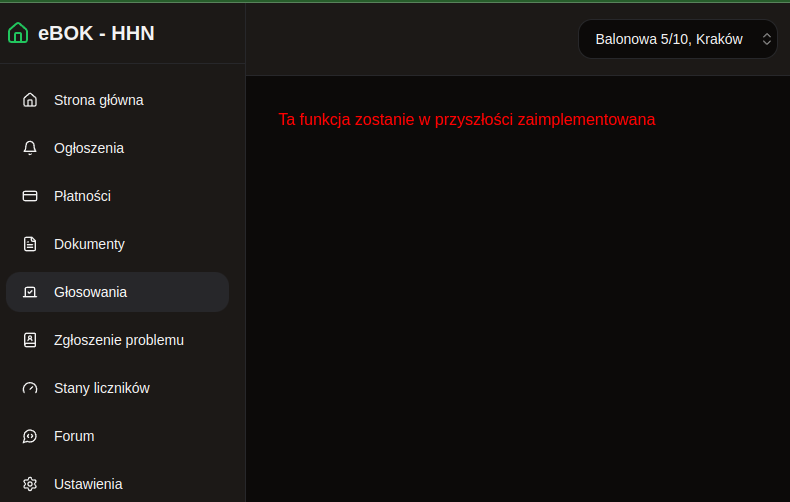
\includegraphics[width=0.63\linewidth]{rys03/poll_ui_unfinish}
    \caption{Aktualny stan UI do głosowań po stronie właściciela.}
    \label{fig:poll_owner_ui}
\end{figure}

Pełny system zarządzania głosowaniami wymagałby zaawansowanych funkcji, takich jak:
\begin{itemize}
    \item \textbf{Automatyczne przypomnienia} -- wysyłanie dynamicznych powiadomień o aktywnych głosowaniach oraz ich wynikach.
    \item \textbf{Wsparcie dla złożonych scenariuszy} -- obsługa głosowań z różnymi rodzajami większości (kwalifikowana, zwykła) oraz indywidualnymi progami.
    \item \textbf{Zaawansowane raportowanie} -- automatyczne generowanie szczegółowych raportów.
    \item \textbf{Integracja z systemami prawnymi i księgowymi} -- automatyczne rejestrowanie wyników głosowań w oficjalnych systemach.
    \item \textbf{Przyjazny interfejs} -- intuicyjna obsługa dla użytkowników, z możliwością przeglądania wyników i śledzenia historii głosowań.
\end{itemize}

%% TO DO: uwaga do diagramów BPMN jak wcześniej !!!!
%%\textbf{Diagramy BPMN} mogą wspierać optymalizację procesów głosowania:
%%\begin{itemize}
    %%\item Graficzne przedstawienie całego procesu, w tym przepływów decyzyjnych i działań uczestników.
    %%\item Analiza i optymalizacja procedur głosowania.
    %%\item Jasne zdefiniowanie ról i odpowiedzialności administratorów, właścicieli mieszkań i systemu.
%%\end{itemize}
%%
%%Dzięki BPMN procesy takie jak organizacja głosowań, przypomnienia oraz analiza wyników mogą być łatwo modelowane i rozwijane zgodnie z wymaganiami wspólnoty.
%%



\section{Systemy zewnętrzne}
System „Harmony Home Net” korzysta z kilku integracji z systemami zewnętrznymi, jednak w prototypie większość z nich została zaimplementowana jako \emph{mocki}, symulujące rzeczywiste działanie. W tej sekcji opisano dostępne integracje oraz ich obecny stan.

\subsection{System bankowości}
Obsługa płatności została uproszczona i zrealizowana przez klasę \texttt{BankingServiceImp}, która symuluje przesyłanie żądania płatności do systemu bankowego. Funkcjonalność ta ogranicza się do wyświetlenia informacji w logach oraz uproszczonego formularza UI właściciela, przedstawionego na rysunku~\ref{fig:mock_of_paymet}.

\begin{figure}[ht]
    \centering
    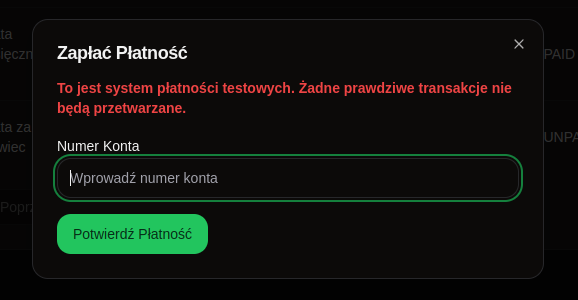
\includegraphics[width=0.63\linewidth]{rys03/mock_pay}
    \caption{Mock formularza płatności}
    \label{fig:mock_of_paymet}
\end{figure}

\begin{lstlisting}[language=Java, style=JavaStyle, caption=Fragment klasy \texttt{BankingServiceImp}]
@Override
public void pay(BigDecimal amount, String account) {
    LOGGER.info("Paying " + amount + " to " + account);
}
\end{lstlisting}

\subsection{System odczytów liczników mediów}
Odczyty wody i prądu są generowane w sposób sztuczny przez klasę \texttt{UtilityMeterServiceImp}. Raz na dobę generuje ona losowe wartości metodą jak niżej.
\begin{lstlisting}[language=Java, style=JavaStyle, caption=Fragment klasy \texttt{UtilityMeterServiceImp}]
@Scheduled(cron = "0 0 0 * * ?")
public void generateRandomMeterReadings() {
    LOG.info("Generating random meter readings");
    waterMeterValue = random.nextDouble() * 1000;
    electricityMeterValue = random.nextDouble() * 1000;
}
\end{lstlisting}

Pewnym wsparciem do obsługi odczytów liczników mogłaby być funkcja przesyłania ich stanów wiadomościami SMS.
\begin{lstlisting}[language=Java, style=JavaStyle, caption=Fragment klasy \texttt{SmsServiceImp}]
@Override
@Async
public void sendSms(String text, String recipient) {
    LOG.info("Sending SMS to " + recipient);
    LOG.info("SMS text: " + text);
}
\end{lstlisting}
Jednak dostęp do rzeczywistych usług SMS wymaga skorzystania z zewnętrznych platform, takich jak Twilio czy Clickatell, które są płatne~\cite{twilio, clickatell}.
Integracja z rzeczywistymi licznikami wymagałaby zaś obsługi odpowiednich urządzeń i ich API.

\subsection{System wysyłania e-maili}

Wysyłanie wiadomości e-mail jest jedynym w pełni funkcjonalnym systemem zewnętrznym w~prototypie. Implementacja korzysta z usługi \texttt{JavaMailSender}, skonfigurowanej do pracy z serwerem Gmail.

\begin{lstlisting}[language=Java, style=JavaStyle, caption=Fragment klasy \texttt{MailServiceImp}]
@Override
@Async
public void sendNotificationMail(String subject, String text, String recipient) {
    try {
        MimeMessage message = mailSender.createMimeMessage();
        MimeMessageHelper helper = new MimeMessageHelper(message, true);

        helper.setTo(recipient);
        helper.setFrom(mailFrom, "Harmony Home Net");
        helper.setSubject(subject);
        helper.setText(text, true);

        mailSender.send(message);
    } catch (Exception ex) {
        throw new RuntimeException("Failed to send email", ex);
    }
}
\end{lstlisting}

Usługa e-maili wymaga konfiguracji konta Gmail oraz przestrzegania jego zasad bezpieczeństwa, takich jak generowanie hasła aplikacji~\cite{gmail_api}.

Poniżej znajduje się fragment kodu konfiguracji \texttt{application.yml}, który definiuje ustawienia dla usługi pocztowej w Spring Boot.

\begin{lstlisting}[language=yaml, caption=Fragment konfiguracji poczty w \texttt{application.yml}]
mail:
  host: smtp.gmail.com
  port: 587
  username: # your email
  password: # your password
  properties:
    mail:
      smtp:
        auth: true
        starttls:
          enable: true
\end{lstlisting}

Znaczenie poszczególnych atrybutów w tej konfiguracji jest następujące:
\begin{itemize}
    \item \texttt{host} -- adres serwera SMTP Gmail.
    \item \texttt{port} -- port używany przez serwer SMTP (587 dla połączeń TLS).
    \item \texttt{username} -- adres e-mail nadawcy.
    \item \texttt{password} -- hasło do konta e-mail (zalecane jest korzystanie z haseł aplikacji).
    \item \texttt{auth} -- włączenie uwierzytelniania SMTP.
    \item \texttt{starttls.enable} -- aktywacja szyfrowania TLS.
\end{itemize}

Zaleca się, aby poufne dane, takie jak hasła, były przechowywane w zaszyfrowanych systemach, takich jak \emph{HashiCorp Vault} lub \emph{AWS Secrets Manager}~\cite{hashicorp_vault, aws_secret}.

\subsection{Typy powiadomień użytkownika}

Użytkownicy mogą wybrać preferowany sposób otrzymywania powiadomień dzięki encji \texttt{NotificationType}. Obsługuje ona dwa rodzaje powiadomień:
\begin{itemize}
    \item \texttt{EMAIL} -- wiadomości e-mail (działające).
    \item \texttt{SMS} -- wiadomości SMS (w trybie \emph{mock}).
\end{itemize}

\noindent Rozbudowa tej funkcji wymaga pełnej integracji z rzeczywistymi systemami komunikacyjnymi.






\section{Testy}
\subsection{Organizacja testów jednostkowych}
W celu zapewnienia wysokiej jakości i niezawodności aplikacji, przeprowadzono testy jednostkowe dla wszystkich głównych serwisów. Implementacja testów opiera się na frameworku JUnit, a testy zostały zorganizowane w odrębnym module aplikacji. Każdy serwis został przetestowany pod kątem poprawności działania metod oraz obsługi wyjątków. Testami weryfikowano:
\begin{itemize}
    \item poprawność logiki biznesowej serwisów,
    \item obsługę wyjątków: \texttt{UserNotFoundException}, \texttt{AnnouncementNotFoundException} itp.,
    \item warunki graniczne dla różnych wartości danych wejściowych.
\end{itemize}

Folder \texttt{serviceTests} zawiera zestawy testów odpowiadające implementacjom serwisów z folderu \texttt{implementation}. Na przykład dla serwisu \texttt{AnnouncementServiceImp} stworzono plik \texttt{AnnouncementServiceTest.java}. Taka struktura pozwala na łatwą nawigację pomiędzy kodem aplikacji a odpowiadającymi mu testami, co usprawnia proces rozwoju i utrzymania.

Przykładowe testy dla serwisu \texttt{AnnouncementService} sprawdzają poprawność działania jego metod, w tym obsługę wyjątków oraz operacje CRUD. Poniżej pokazano wybrane fragmenty kodu testów. Testy te sprawdzają:
\begin{itemize}
    \item obsługę błędów, np. brak zasobu w bazie danych,
    \item poprawność zapisu nowych danych,
    \item skuteczność usuwania rekordów z bazy danych.
\end{itemize}

\begin{lstlisting}[language=Java, style=JavaStyle, caption= Przykłądowe testy dla \texttt{AnnouncementService}]
@Test
void testFindAnnouncementById_NotFound() {
    when(announcementRepository.findById(anyLong())).thenReturn(Optional.empty());
    Assertions.assertThrows(AnnouncementNotFoundException.class, () -> {
        announcementService.findAnnouncementById(1L);
    });
}

@Test
void testCreateAnnouncement_Success() {
    Announcement announcement = new Announcement("New Announcement", "Description");
    when(announcementRepository.save(any(Announcement.class))).thenReturn(announcement);
    Announcement result = announcementService.createAnnouncement(announcement);
    Assertions.assertEquals("New Announcement", result.getTitle());
}

@Test
void testDeleteAnnouncementById_Success() {
    doNothing().when(announcementRepository).deleteById(anyLong());
    Assertions.assertDoesNotThrow(() -> {
        announcementService.deleteAnnouncementById(1L);
    });
}
\end{lstlisting}



\subsection{Wyniki testów jednostkowych}
Wszystkie testy jednostkowe zakończyły się pozytywnie, co potwierdza, że zaimplementowane serwisy działają zgodnie z założeniami. Pokrycie testami obejmuje główne przypadki użycia aplikacji. Na rysunku~\ref{fig:test_presetation} przedstawiono fragmenty wyników dwóch serii testów.

\begin{figure}[htb]
	\centering
		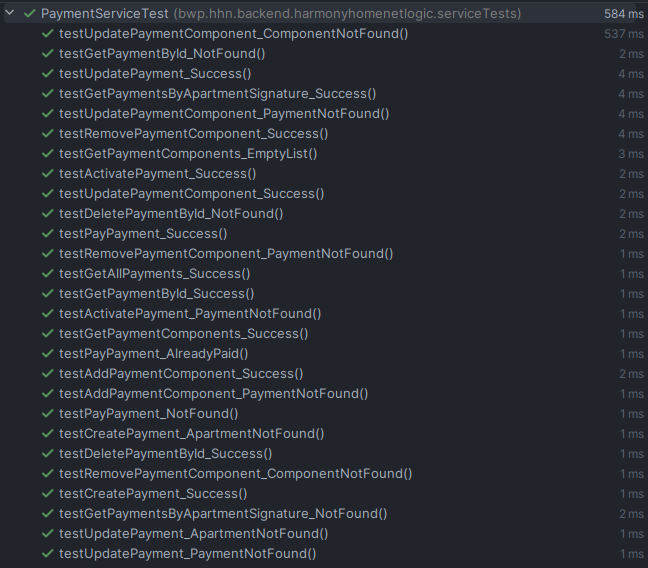
\includegraphics[width=0.91\linewidth]{rys03/testy/platnosci_testy} 
		\\
		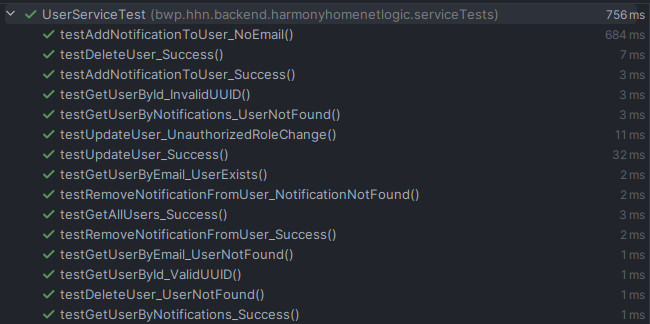
\includegraphics[width=0.91\linewidth]{rys03/testy/user_testy} 
		\caption{Przedstawienie 2 serii testów dla systemu}
	\label{fig:test_presetation}
\end{figure}

